%% bare_conf_compsoc.tex
%% V1.4b
%% 2015/08/26
%% by Michael Shell
%% See:
%% http://www.michaelshell.org/
%% for current contact information.
%%
%% This is a skeleton file demonstrating the use of IEEEtran.cls
%% (requires IEEEtran.cls version 1.8b or later) with an IEEE Computer
%% Society conference paper.
%%
%% Support sites:
%% http://www.michaelshell.org/tex/ieeetran/
%% http://www.ctan.org/pkg/ieeetran
%% and
%% http://www.ieee.org/

%%*************************************************************************
%% Legal Notice:
%% This code is offered as-is without any warranty either expressed or
%% implied; without even the implied warranty of MERCHANTABILITY or
%% FITNESS FOR A PARTICULAR PURPOSE! 
%% User assumes all risk.
%% In no event shall the IEEE or any contributor to this code be liable for
%% any damages or losses, including, but not limited to, incidental,
%% consequential, or any other damages, resulting from the use or misuse
%% of any information contained here.
%%
%% All comments are the opinions of their respective authors and are not
%% necessarily endorsed by the IEEE.
%%
%% This work is distributed under the LaTeX Project Public License (LPPL)
%% ( http://www.latex-project.org/ ) version 1.3, and may be freely used,
%% distributed and modified. A copy of the LPPL, version 1.3, is included
%% in the base LaTeX documentation of all distributions of LaTeX released
%% 2003/12/01 or later.
%% Retain all contribution notices and credits.
%% ** Modified files should be clearly indicated as such, including  **
%% ** renaming them and changing author support contact information. **
%%*************************************************************************


% *** Authors should verify (and, if needed, correct) their LaTeX system  ***
% *** with the testflow diagnostic prior to trusting their LaTeX platform ***
% *** with production work. The IEEE's font choices and paper sizes can   ***
% *** trigger bugs that do not appear when using other class files.       ***                          ***
% The testflow support page is at:
% http://www.michaelshell.org/tex/testflow/



\documentclass[conference,compsoc]{IEEEtran}
% Some/most Computer Society conferences require the compsoc mode option,
% but others may want the standard conference format.
%
% If IEEEtran.cls has not been installed into the LaTeX system files,
% manually specify the path to it like:
% \documentclass[conference,compsoc]{../sty/IEEEtran}





% Some very useful LaTeX packages include:
% (uncomment the ones you want to load)


% *** MISC UTILITY PACKAGES ***
%
%\usepackage{ifpdf}
% Heiko Oberdiek's ifpdf.sty is very useful if you need conditional
% compilation based on whether the output is pdf or dvi.
% usage:
% \ifpdf
%   % pdf code
% \else
%   % dvi code
% \fi
% The latest version of ifpdf.sty can be obtained from:
% http://www.ctan.org/pkg/ifpdf
% Also, note that IEEEtran.cls V1.7 and later provides a builtin
% \ifCLASSINFOpdf conditional that works the same way.
% When switching from latex to pdflatex and vice-versa, the compiler may
% have to be run twice to clear warning/error messages.






% *** CITATION PACKAGES ***
%
\ifCLASSOPTIONcompsoc
  % IEEE Computer Society needs nocompress option
  % requires cite.sty v4.0 or later (November 2003)
  \usepackage[nocompress]{cite}
\else
  % normal IEEE
  \usepackage{cite}
\fi
% cite.sty was written by Donald Arseneau
% V1.6 and later of IEEEtran pre-defines the format of the cite.sty package
% \cite{} output to follow that of the IEEE. Loading the cite package will
% result in citation numbers being automatically sorted and properly
% "compressed/ranged". e.g., [1], [9], [2], [7], [5], [6] without using
% cite.sty will become [1], [2], [5]--[7], [9] using cite.sty. cite.sty's
% \cite will automatically add leading space, if needed. Use cite.sty's
% noadjust option (cite.sty V3.8 and later) if you want to turn this off
% such as if a citation ever needs to be enclosed in parenthesis.
% cite.sty is already installed on most LaTeX systems. Be sure and use
% version 5.0 (2009-03-20) and later if using hyperref.sty.
% The latest version can be obtained at:
% http://www.ctan.org/pkg/cite
% The documentation is contained in the cite.sty file itself.
%
% Note that some packages require special options to format as the Computer
% Society requires. In particular, Computer Society  papers do not use
% compressed citation ranges as is done in typical IEEE papers
% (e.g., [1]-[4]). Instead, they list every citation separately in order
% (e.g., [1], [2], [3], [4]). To get the latter we need to load the cite
% package with the nocompress option which is supported by cite.sty v4.0
% and later.






% *** GRAPHICS RELATED PACKAGES ***
%
\ifCLASSINFOpdf
  \usepackage[pdftex]{graphicx}
  % declare the path(s) where your graphic files are
  % \graphicspath{{../pdf/}{../jpeg/}}
  % and their extensions so you won't have to specify these with
  % every instance of \includegraphics
  % \DeclareGraphicsExtensions{.pdf,.jpeg,.png}
\else
  % or other class option (dvipsone, dvipdf, if not using dvips). graphicx
  % will default to the driver specified in the system graphics.cfg if no
  % driver is specified.
  \usepackage[dvips]{graphicx}
  % declare the path(s) where your graphic files are
  % \graphicspath{{../eps/}}
  % and their extensions so you won't have to specify these with
  % every instance of \includegraphics
  % \DeclareGraphicsExtensions{.eps}
\fi
% graphicx was written by David Carlisle and Sebastian Rahtz. It is
% required if you want graphics, photos, etc. graphicx.sty is already
% installed on most LaTeX systems. The latest version and documentation
% can be obtained at: 
% http://www.ctan.org/pkg/graphicx
% Another good source of documentation is "Using Imported Graphics in
% LaTeX2e" by Keith Reckdahl which can be found at:
% http://www.ctan.org/pkg/epslatex
%
% latex, and pdflatex in dvi mode, support graphics in encapsulated
% postscript (.eps) format. pdflatex in pdf mode supports graphics
% in .pdf, .jpeg, .png and .mps (metapost) formats. Users should ensure
% that all non-photo figures use a vector format (.eps, .pdf, .mps) and
% not a bitmapped formats (.jpeg, .png). The IEEE frowns on bitmapped formats
% which can result in "jaggedy"/blurry rendering of lines and letters as
% well as large increases in file sizes.
%
% You can find documentation about the pdfTeX application at:
% http://www.tug.org/applications/pdftex





% *** MATH PACKAGES ***
%
\usepackage{amsmath}
% A popular package from the American Mathematical Society that provides
% many useful and powerful commands for dealing with mathematics.
%
% Note that the amsmath package sets \interdisplaylinepenalty to 10000
% thus preventing page breaks from occurring within multiline equations. Use:
%\interdisplaylinepenalty=2500
% after loading amsmath to restore such page breaks as IEEEtran.cls normally
% does. amsmath.sty is already installed on most LaTeX systems. The latest
% version and documentation can be obtained at:
% http://www.ctan.org/pkg/amsmath





% *** SPECIALIZED LIST PACKAGES ***
%
\usepackage{algorithmic}
\usepackage{algorithm}
% algorithmic.sty was written by Peter Williams and Rogerio Brito.
% This package provides an algorithmic environment fo describing algorithms.
% You can use the algorithmic environment in-text or within a figure
% environment to provide for a floating algorithm. Do NOT use the algorithm
% floating environment provided by algorithm.sty (by the same authors) or
% algorithm2e.sty (by Christophe Fiorio) as the IEEE does not use dedicated
% algorithm float types and packages that provide these will not provide
% correct IEEE style captions. The latest version and documentation of
% algorithmic.sty can be obtained at:
% http://www.ctan.org/pkg/algorithms
% Also of interest may be the (relatively newer and more customizable)
% algorithmicx.sty package by Szasz Janos:
% http://www.ctan.org/pkg/algorithmicx




% *** ALIGNMENT PACKAGES ***
%
%\usepackage{array}
% Frank Mittelbach's and David Carlisle's array.sty patches and improves
% the standard LaTeX2e array and tabular environments to provide better
% appearance and additional user controls. As the default LaTeX2e table
% generation code is lacking to the point of almost being broken with
% respect to the quality of the end results, all users are strongly
% advised to use an enhanced (at the very least that provided by array.sty)
% set of table tools. array.sty is already installed on most systems. The
% latest version and documentation can be obtained at:
% http://www.ctan.org/pkg/array


% IEEEtran contains the IEEEeqnarray family of commands that can be used to
% generate multiline equations as well as matrices, tables, etc., of high
% quality.




% *** SUBFIGURE PACKAGES ***
% \ifCLASSOPTIONcompsoc
%  \usepackage[caption=false,font=footnotesize,labelfont=sf,textfont=sf]{subfig}
% \else
%  \usepackage[caption=false,font=footnotesize]{subfig}
% \fi
\usepackage[caption=false,font=footnotesize]{subfig}
% subfig.sty, written by Steven Douglas Cochran, is the modern replacement
% for subfigure.sty, the latter of which is no longer maintained and is
% incompatible with some LaTeX packages including fixltx2e. However,
% subfig.sty requires and automatically loads Axel Sommerfeldt's caption.sty
% which will override IEEEtran.cls' handling of captions and this will result
% in non-IEEE style figure/table captions. To prevent this problem, be sure
% and invoke subfig.sty's "caption=false" package option (available since
% subfig.sty version 1.3, 2005/06/28) as this is will preserve IEEEtran.cls
% handling of captions.
% Note that the Computer Society format requires a sans serif font rather
% than the serif font used in traditional IEEE formatting and thus the need
% to invoke different subfig.sty package options depending on whether
% compsoc mode has been enabled.
%
% The latest version and documentation of subfig.sty can be obtained at:
% http://www.ctan.org/pkg/subfig




% *** FLOAT PACKAGES ***
%
%\usepackage{fixltx2e}
% fixltx2e, the successor to the earlier fix2col.sty, was written by
% Frank Mittelbach and David Carlisle. This package corrects a few problems
% in the LaTeX2e kernel, the most notable of which is that in current
% LaTeX2e releases, the ordering of single and double column floats is not
% guaranteed to be preserved. Thus, an unpatched LaTeX2e can allow a
% single column figure to be placed prior to an earlier double column
% figure.
% Be aware that LaTeX2e kernels dated 2015 and later have fixltx2e.sty's
% corrections already built into the system in which case a warning will
% be issued if an attempt is made to load fixltx2e.sty as it is no longer
% needed.
% The latest version and documentation can be found at:
% http://www.ctan.org/pkg/fixltx2e


%\usepackage{stfloats}
% stfloats.sty was written by Sigitas Tolusis. This package gives LaTeX2e
% the ability to do double column floats at the bottom of the page as well
% as the top. (e.g., "\begin{figure*}[!b]" is not normally possible in
% LaTeX2e). It also provides a command:
%\fnbelowfloat
% to enable the placement of footnotes below bottom floats (the standard
% LaTeX2e kernel puts them above bottom floats). This is an invasive package
% which rewrites many portions of the LaTeX2e float routines. It may not work
% with other packages that modify the LaTeX2e float routines. The latest
% version and documentation can be obtained at:
% http://www.ctan.org/pkg/stfloats
% Do not use the stfloats baselinefloat ability as the IEEE does not allow
% \baselineskip to stretch. Authors submitting work to the IEEE should note
% that the IEEE rarely uses double column equations and that authors should try
% to avoid such use. Do not be tempted to use the cuted.sty or midfloat.sty
% packages (also by Sigitas Tolusis) as the IEEE does not format its papers in
% such ways.
% Do not attempt to use stfloats with fixltx2e as they are incompatible.
% Instead, use Morten Hogholm'a dblfloatfix which combines the features
% of both fixltx2e and stfloats:
%
% \usepackage{dblfloatfix}
% The latest version can be found at:
% http://www.ctan.org/pkg/dblfloatfix




% *** PDF, URL AND HYPERLINK PACKAGES ***
%
\usepackage{url}
% url.sty was written by Donald Arseneau. It provides better support for
% handling and breaking URLs. url.sty is already installed on most LaTeX
% systems. The latest version and documentation can be obtained at:
% http://www.ctan.org/pkg/url
% Basically, \url{my_url_here}.




% *** Do not adjust lengths that control margins, column widths, etc. ***
% *** Do not use packages that alter fonts (such as pslatex).         ***
% There should be no need to do such things with IEEEtran.cls V1.6 and later.
% (Unless specifically asked to do so by the journal or conference you plan
% to submit to, of course. )

%\usepackage[utf8]{inputenc}

%\usepackage{natbib}
%\usepackage{indentfirst}
\usepackage{listings}
%\usepackage{caption}
%\usepackage{subcaption}






% correct bad hyphenation here
\hyphenation{op-tical net-works semi-conduc-tor}


\begin{document}
%
% paper title
% Titles are generally capitalized except for words such as a, an, and, as,
% at, but, by, for, in, nor, of, on, or, the, to and up, which are usually
% not capitalized unless they are the first or last word of the title.
% Linebreaks \\ can be used within to get better formatting as desired.
% Do not put math or special symbols in the title.
\title{Interactional Justice: finding consensus in the multitude of claims}

% author names and affiliations
% use a multiple column layout for up to three different
% affiliations
\author{\IEEEauthorblockN{David Kurka and Jeremy Pitt}
\IEEEauthorblockA{Department of Electrical and Electronic Engineering\\
Imperial College London\\
Exhibition Road, London, SW7 2BT, UK\\
Email: \{d.kurka, j.pitt\}@imperial.ac.uk}}

% conference papers do not typically use \thanks and this command
% is locked out in conference mode. If really needed, such as for
% the acknowledgment of grants, issue a \IEEEoverridecommandlockouts
% after \documentclass

% for over three affiliations, or if they all won't fit within the width
% of the page (and note that there is less available width in this regard for
% compsoc conferences compared to traditional conferences), use this
% alternative format:
% 
%\author{\IEEEauthorblockN{Michael Shell\IEEEauthorrefmark{1},
%Homer Simpson\IEEEauthorrefmark{2},
%James Kirk\IEEEauthorrefmark{3}, 
%Montgomery Scott\IEEEauthorrefmark{3} and
%Eldon Tyrell\IEEEauthorrefmark{4}}
%\IEEEauthorblockA{\IEEEauthorrefmark{1}School of Electrical and Computer Engineering\\
%Georgia Institute of Technology,
%Atlanta, Georgia 30332--0250\\ Email: see http://www.michaelshell.org/contact.html}
%\IEEEauthorblockA{\IEEEauthorrefmark{2}Twentieth Century Fox, Springfield, USA\\
%Email: homer@thesimpsons.com}
%\IEEEauthorblockA{\IEEEauthorrefmark{3}Starfleet Academy, San Francisco, California 96678-2391\\
%Telephone: (800) 555--1212, Fax: (888) 555--1212}
%\IEEEauthorblockA{\IEEEauthorrefmark{4}Tyrell Inc., 123 Replicant Street, Los Angeles, California 90210--4321}}




% use for special paper notices
%\IEEEspecialpapernotice{(Invited Paper)}




% make the title area
\maketitle

% As a general rule, do not put math, special symbols or citations
% in the abstract
\begin{abstract}

\end{abstract}

% no keywords




% For peer review papers, you can put extra information on the cover
% page as needed:
% \ifCLASSOPTIONpeerreview
% \begin{center} \bfseries EDICS Category: 3-BBND \end{center}
% \fi
%
% For peerreview papers, this IEEEtran command inserts a page break and
% creates the second title. It will be ignored for other modes.
\IEEEpeerreviewmaketitle


\maketitle

\section{Introduction}

Resource allocation in networks has been a subject of interest from both industry and academia. The considerable and intense increase of connected systems, such as smart grids, cellular networks and cloud computing, motivates and challenges the development of increasingly better strategies, able to deal with new demands.

Previous work explore effective policies of resource allocation in scarcity environments, using decentralised and self-organised approaches \cite{Pitt2012Distributive,Pitt2015Pursuit}. By using principles first observed in human societies \cite{Ostrom1990}, it is possible to create schemes where socio-technical multi-agent systems act in fair ways, collectively achieving what is defined as \emph{computational justice}.

Notwithstanding the positive and practical results already found, some open questions still arise and can be explored. The most evident one concerns the mechanisms used to verify the proper functioning of a current policy.

In the current solutions, clusters of agents come together to collective decide the criteria with which resources should be distributed among its members, using voting processes. However, each cluster have one distinguished agent, the \emph{head}, who is responsible for actually executing actions for the (collectively) decided resource allocation policy, such as counting votes and distributing resources.


Although the presence of this distinct role is necessary in order to allow the actual execution of policies, it can also leads to failures, if there is any problem with the execution process (either by malfunction or malice).

The problem that arises and motivates this present work is whether there are mechanisms to avoid problems with the head procedures. Ideally, such mechanism should be developed within members of a cluster and take into consideration possible failures or malicious intentions of every component of this process. There is also the motivation for strategies that do not compromise the decentralised and parallel nature of the original strategies by introducing expensive or blocking computations (e.g.\ a solution where every agent fully monitors all the others can be very effective, but also very limiting by its costs).


This work will explore a framework of interactional justice, where agents subject to an allocation policy, communicating its own individual and subjective perspectives of fairness, find mechanisms able to create general mobilisations and perceptions of possible problems that take place in the network. Such mobilisations can serve as indications of malfunctioning of a network and be the first process of a process of change in the system and assist the quest for the permanence of fair systems.
%The mechanisms will also seek to be fair by itself, i.e. 

\section{Problem formulation}

\noindent
\textbf{Environment setup}

Consider a cluster of $n$ agents, with connections defined by an undirected graph $G = \{E,V\}$. One specific member of the cluster is designed as \emph{head} and is responsible for defining the allocation of resources, for every agent of the cluster (including itself).

The process work in turns. At each turn $t$, each agent $i$ has a specific demand, denoted $d_i$, and there is an defined amount of resources $P_t$. The amount of resources per turn is smaller than the total demand ($P_t < \sum_i d_i$ ), creating an scarcity environment.

Given a turn's amount of resources and the demands distribution, the head of the cluster will then, using an allocation policy, define individuals attributions ($r_i$). The chosen allocation policy can be considered fair or not, depending on the amount of resources given to the agents over time.

\noindent
\textbf{Information disclosure}

Each agent $i$ has a neighbourhood ($\mathcal{N}_i$), defined as the list of adjacent vertices of $i$ in graph $G$. Every agent can see its own demands ($d_i$) and allocated resources ($r_i$) overtime and also its neighbours. 

\noindent
\textbf{Metrics of satisfaction}

Every agent also develop a measurement of  \emph{perceived fairness} over time ($\phi_i(t)$), which is influenced both by its individual and local perceptions of how resources are being allocated. An agent can also observe its neighbours perceived fairness.

Individual perceptions of fairness can be grouped, resulting into an \emph{collective perceived fairness} $\Phi(t)$, that can be used as a metric for general satisfaction.

\noindent
\textbf{Problem Statement}

Given the execution of a resource allocation policy by a head in a cluster, how the interactions of the agents in a cluster can help to access the fairness of it?


\section{Towards an Interactional Justice Framework}

The Interactional Justice framework proposed to deal with this problem, consists in using individual subjective assessments of fairness, in order to achieve a global sense of justice that can be really representative of the system.

There are some clear positive aspects of this strategy:
\begin{itemize}
    \item It allows the independent assessment of a (supposedly) same truth, shared by many witnesses, increasing the reliability of the process (wisdom of the crowds);
    \item Inherent decentralisation of the process, as subjectively impressions can be made independently and autonomously;
    \item Gives voice to ``normal'' individuals that might be subject to a unfair treatment by the head.
\end{itemize}


But also some challenges:
\begin{itemize}
    \item How to deal with malicious agent that try to manipulate its individual opinions, in order to harm a head?
    \item How to weight opinions, in case of discordance of opinions?
\end{itemize}

Those points are used as guidelines to the development of a solution.

\subsection{Algorithm}

A simple algorithm is sketched below. Every turn, the following steps are processed, resulting in an output of

\begin{verbatim}
1. Allocation 
2. Reaction (perceived fairness)
2.1 Formulation of personal opinions
2.2 Comparison to environment (trust)
2.3 Diffusion of opinions
3. Aggregate personal perceptions
\end{verbatim}


\subsubsection*{Allocation}

Head, following a certain policy, define the resources each agent will receive in a given turn. Six possibilities are explored:


\begin{itemize}
    \item \textbf{average fair}: serve all individuals with the same frequency.
    \item \textbf{clique first}: serve first a fixed `elite' group (or `cartel') chosen by the head and then (if there are any remaining resources) the others.
    \item \textbf{random order}: draw an order of service every turn.
    \item \textbf{ration}: give the same amount to all individuals.
\end{itemize}



\subsubsection*{Formulation of personal opinions}

Each individual, in light of the amount of resources received over time and the amount of resources demanded, can elaborate a personal opinion of the fairness of an allocation method.

The evaluation of the fairness of a distributive process is a complex topic discussed over years in the social sciences literature. On this topic, Nicholas Rescher \cite{Rescher1969} explore different principles commonly used to measure the justice of a distributive processes. Those principles are denominated as \emph{legitimate claims} of justice.

According to Rescher \cite{Rescher1969}, a diversity of legitimate claims should be used to evaluate a system, allowing the emergence of a plurality of interpretations that can be compared, weighted and jointly evaluated. Still in his work, seven legitimate claims are enumerated and discussed.

In light of Rescher's work, Pitt et al.\ \cite{Pitt2012Distributive} build a formal characterisation of the claims, translating them to mathematical and logical notation.

Many of the metrics defined in \cite{Pitt2012Distributive} can also be used in the present context, as measurements of fairness. Below are presented the metrics used and its correspondent claims of justice. In all expressions, $T$ is the number of rounds individual $i$ has been under a specific allocation policy.

\noindent
\textbf{Canons of equality:}

\begin{equation}
  \phi_{i}^{1}(T) = \frac{\displaystyle \sum_{t=0}^T \left ( r_i(t) \geq d_i(t) \right )}{T}
\label{opinion_percentage}  
\end{equation}

\begin{equation}
  \phi_{i}^{2}(T) = \frac{\displaystyle \sum_{t=0}^T \left ( r_i(t) \right )}{T}
\label{opinion_received}  
\end{equation}

\begin{equation}
 \phi_{i}^{3}(T) = 
  \begin{cases} 
  (1 - \alpha) \cdot \phi_{i}^{3}(T-1) +  \alpha & \text{if } r_i(T) \geq d_i(T)\\
  (1 - \beta) \cdot \phi_{i}^{3}(T-1)  & \text{if } r_i(T) < d_i(T)
  \end{cases}
\label{opinion_sat}
\end{equation}

(Eq. \ref{opinion_sat} is also called \emph{satisfaction index} and $\alpha$ and $\beta$ are respectively positive and negative reinforcement rates and can be adjusted to represent the level of optimism/pessimism of individual agents, to system changes.)



% However, a metric that can take into consideration the temporal natural of the distribution of the distribution (and not just the average) can also reveal other interesting aspects of a policy (un)fairness. A useful metric that fits this purpose, proposed in \cite{Pitt2012Distributive} is the \emph{satisfaction index} given by:

\noindent
\textbf{Canon of needs:}

\begin{equation}
  \phi_{i}^{4}(T) = \frac{\displaystyle \sum_{t=0}^T \left ( 1 - \frac{d_i(t) - d_{\textit{min}}(t)}{d_{\textit{max}}(t) - d_{\textit{min}}(t)} \right )}{T}
\label{opinion_demand}  
\end{equation}


Note that canons 3-7 (canon of productivity, canon of effort, canon of social utility, canon of supply and demand and canon of merit and achievements) are not used here, for not having clear applications, given the problem formulation.

Given the multiple perspectives of each individual, regarding the justice of the system, it is possible then combine them as a linear combination, obtaining a \emph{personal opinion} $\phi_i(T)$:


\begin{equation}
  \phi_{i}(T) = \sum_{*=1}^{4} w_{*} \cdot \phi_{i}^{*}(T)
\label{opinion_gen}  
\end{equation}

The weights $w_i, i \in \{1, \dots 4\}$ can be defined to give different importance for each metric.



\subsubsection*{Comparison to environment - trust assessment}

Having formulated its personal opinion, agents then start to observe each other opinions, in order to compare their assessments.

This comparison is important as the knowledge of each individual is limited to its context and, by observing its neighbours, information of the environment of more distant areas of the network can be obtained and contribute to a more realistic impression of what is happening in the network in general.

Therefore, a mechanism for updating an individual opinion, given its contact to different opinions should be developed. However, before exploring the transmission of information, one important issue should be considered: how to conciliate and ponder multiple independent accounts.

Specially in scenarios where there is discrepancy among neighbour's opinions, there should be ways of weighting the relevance of each received account. Also, considering that unfairness and cheating behaviour can be present in the system dynamics, each individual should develop ways of protecting itself from false accounts and find impressions as close to the truth as possible.


In \cite{Neville}, Neville and Pitt introduce the important concept of \emph{trust} in multi-agent systems. In their formalisation, a framework is built where agents subject to a trust decision towards other agent take into consideration two main factors: (a) a subjective confidence, based on the analysis of past interactions (socio-cognitive aspect) and (b) the direct benefits that a relationship of trust can bring (socio-economic aspects).
Therefore, trust is a function of not only past experiences, but also the personal benefits in interacting with an agent, even if its known that he is cheating.

%TODO: image of trust framework


Another interesting concept, discussed in \cite{PittDagostino}, is the use of \emph{scoring rules} as a way of measuring agents reputation and assuring that agents' claims are consistent to their actual experiences. A scoring rule is a function, $S(\phi_i(t), R_i, D_i)$, that takes into consideration an agent's claimed opinion ($\phi_i(t)$) and the history of resources received ($R_i = \sum R_i (t)$) and demanded ($D_i = \sum d_i(t)$), returning an index. The function is defined in such a way that if the agent's opinion is in accordance to its reality, the returned index is high; if an opinion is discrepant to its context, then a low index is returned.


Taking these concepts into consideration, we aim to build a metric that define the trust ($T_{i,j}$) of agent $i$ in $j$.

Initially, a metric is defined to determine the divergence of opinions in a given time. For this, we define an \emph{accordance index} $\tau_{ij}(t)$ as a value in the range $[0,1]$, representing the level of ``agreement'' between two individuals ($i$ and $j$) at timestamp $t$.


A initial simple definition of $\tau$ can be given solely by the difference of opinions of $i$ and $j$:

\begin{equation}
  \tau_{ij}(t) = 1 - | \phi_i(t) - \phi_j(t) |
\label{trust_my}
\end{equation}

Eq. \ref{trust_my} can be improved with more information, if we consider not only agent $i$'s perception, but also its context, given by $i$ neighbours' opinions:

\begin{equation}
  \tau_{ij}(t) = 1 - |\bar\phi_{N_i}(t) - \phi_j(t) |
\end{equation}

where:

$$\bar\phi_{N_i}(t) = \frac{1}{|\text{Neighbours}(i)|} \sum_{n \in \text{Neighbours}(i)-\{j\}+\{i\}} \phi_n(t)$$


Extending even more $\tau$, we can develop a function where the difference of opinions can be attenuated or amplified, depending on its magnitude. One example of such function is the logistic function defined as:

\begin{equation}
  \tau_{ij}(t) = 1 - \frac{1}{1 + e^{-k(|\bar\phi_{N_i}(t) - \phi_j(t) | - \epsilon_0)}}
\label{logistic}
\end{equation}

where $k$ is a coefficient defining the steepness of the transient curve and $\epsilon_0$ is the midpoint of the curve, representing a threshold for the difference of opinions before the accordance goes rapidly to 0.

%plotar a funcao logistica

given individual's difference of opinions,
Note that all definition of $\tau$ extract elements of \cite{Neville}, as individuals that agree with each other tend to trust in each other, turning trust into a function of reinforcement of personal opinions and self benefit.

However, aspects concerning individuals past experiences and agents' reputation should also be considered. In the light of \cite{PittDagostino} scoring rules, we then formulate the definition of $T_{ij}(t)$ as a function of previous trust assessments ($T_{i,j}(t-1)$) and the current accordance ($\tau_{ij}(t)$):

\begin{equation}
    T_{i,j}(t) = (1 - \gamma) \cdot T_{i,j} \left ( t-1 \right ) +  \gamma \cdot \tau_{ij}(t)
    \label{trust}
\end{equation}

where $\gamma$ is a defined reinforcement rate.



% Given a number of turns $t$, the percentage of rounds that agent $j$ was served  $\phi_j(t)$ (defined as in Eq. \ref{opinion_percentage}), and the mean number of rounds that $i$ has observed agents being served among its neighbours $\text{fair\_obs}_i(t)$, we define the likelihood function:


% \begin{equation}
%     T_{i,j} = P(obs_i | \phi_j) = \binom{\text{n\_obs}_i}{\text{fair\_obs}_i} \phi_j^{\text{n\_obs}_i} (1-\phi_j)^{\text{n\_obs}_i-\text{fair\_obs}_i}
%     \label{trust_likelihood}
% \end{equation}

Having defined an accordance index (from the options above), it is possible to build a matrix $T$ at each time-step, formed by values of $T_{i,j}(t)$ for all combinations of individuals $i$ and $j$. Note that, when $i$ and $j$ do not have connections in $G$, $T_{i,j}$ should be $0$. Also, every row of T should be normalised by its sum, so the line $i$ in matrix $T$ have a probability distribution with sum $1$, representing the trust distribution of agent $i$ in all cluster members.


\subsubsection*{Diffusion of opinions}


Having the personal opinions $\phi$ and the trust matrix $T$ we can model the evolution of opinions under social influence. The idea is that, when an agent is in a context of divergence of opinions, he will update his own initial opinion, using its neighbours opinions and reputations.

One approach to model this process is given in \cite{degott}, where an opinion vector can be updated through a iterative process of influence, by multiplying the matrix $T$ over vector $\phi$ multiple times, obtaining the updated opinion vector $\phi'$:

\begin{equation}
  \phi' = T^{K}\phi   
\end{equation}
where $K$ is a number of iterations, generally big enough to allow convergence.

\begin{figure}
    \centering
    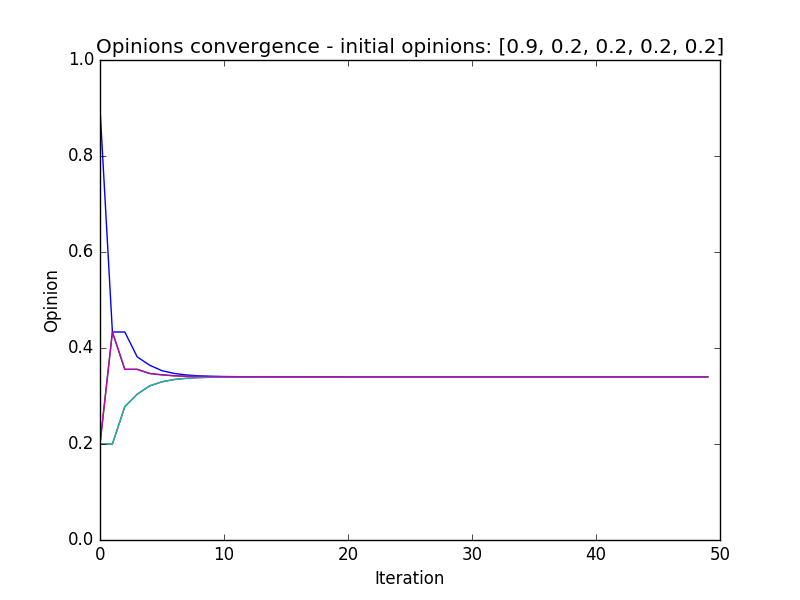
\includegraphics[width=0.8\linewidth]{pics/trust_progression.png}
    \caption{Example of trust progression, using DeGroot algorithm.}
    \label{fig:deGroot}
\end{figure}


Ramirez-Cano and Pitt \cite{Ramirez-Cano2006} also explore this problem, suggesting an alternative method where, differently from \cite{degott}, the matrix $T$ is updated at each of the $k$ iterations. In this approach, a matrix $T(0)$ is first initialised with predefined trust values and, at each iteration, $T_{ij}$ is strengthened if $j$'s current opinion is closer to $i$'s original opinion and weakened otherwise. The function for computing distance between opinions is equivalent to Eq. \ref{trust_my} and is denominated \emph{affinity} ($a_{ij}$).

Therefore, using this method, it is possible to obtain an updated opinion vector as:

\begin{equation}
    \phi' = \prod_k^K T(k) \cdot \phi \\
\end{equation}

Where:
$$
T_{ij}(k) = \frac{T_{ij}(k-1) + T_{ij}(k-1) a_{ij}(k-1)}{\sum_{l=1}^n \left ( T_{il}(k-1) + T_{il}(k-1) a_{il}(k-1) \right ) }
$$


%TODO: comparison between two methods (graph of converging opinions


%In both methods, the determination of a trust function is the most important aspect

\subsubsection*{Aggregate personal perceptions}

Finally, in order to compute a simple average of each individual opinion (after influence process):

$$\Phi(t) = \frac{1}{n}\sum_i \phi'_i(t)$$

\subsection{Pseudocode}

Bellow, all the steps described in the previous section are summarised in code:


\begin{algorithm}
\caption{Complete algorithm}
\begin{algorithmic}[1]
\STATE $\phi_i \leftarrow 0.5 \qquad \forall i \in \text{Agents}$
\STATE $t \leftarrow 0$
\REPEAT
    \STATE \COMMENT{1. Allocation}
    \FOR{each $i \in \text{Agents}$}
        \STATE $D_i(t) \leftarrow \text{demand}(i)$ 
        \STATE $R_i(t) \leftarrow \text{allocate}(i, \text{policy}(h))$ 
    \ENDFOR
    \STATE \COMMENT{2. Reaction (perceived fairness)}
    \STATE \COMMENT{2.1 Formulation of personal opinions}
    \FOR{each $i \in \text{Agents}$}
        \FOR{each $\text{c} \in \text{Canons}$}
            \STATE $\phi_{i}^{c}(t) \leftarrow \text{compute\_canon}(c)$
        \ENDFOR
        \STATE $\phi_i(t) \leftarrow \sum_c w_c \cdot \phi_{i}^{c}(t)$
    \ENDFOR
    \STATE \COMMENT{2.2 Trust assessments}
    \FOR{each $i \in \text{Agents}$}
        \FOR{each $j \in \text{Agents}$}
            \IF {$j \in i.\text{neighbours}$}
                \STATE $\tau_{ij}(t) \leftarrow \text{accordance}(\phi_j(t), \bar\phi_{N_i}(t))$
                \STATE $T_{ij}(t) \leftarrow (1-\gamma) T_{ij}(t-1) + \gamma \tau_{ij}(t) $
            \ELSE 
                \STATE $T_{ij}(t) \leftarrow 0 $
            \ENDIF
        \ENDFOR
    \ENDFOR
    
    
    \STATE \COMMENT{2.3 Diffusion of opinions}
    \STATE $\phi \leftarrow \phi(t)$
    \FOR{$k=0$ to $K$}
        \STATE $\phi' \leftarrow T \times \phi$
        \STATE $\phi \leftarrow \phi'$
    \ENDFOR
    \STATE $\phi'(t) \leftarrow \phi'$
    \STATE \COMMENT{3. Aggregate personal perceptions}
    \STATE $\Phi(t) \leftarrow \frac{\sum_i \phi'_i(t)}{|\text{Agents}|}$
\UNTIL{$t == \text{lim\_turns}$}


% \STATE $y \leftarrow 1$
% \STATE $X \leftarrow x$
% \STATE $N \leftarrow n$
% \WHILE{$N \neq 0$}
% \IF{$N$ is even}
% \STATE $X \leftarrow X \times X$
% \STATE $N \leftarrow N / 2$
% \ELSE[$N$ is odd]
% \STATE $y \leftarrow y \times X$
% \STATE $N \leftarrow N - 1$
% \ENDIF
% \ENDWHILE
\end{algorithmic}
\end{algorithm}

% \begin{minipage}{\linewidth}
% \begin{lstlisting}[language=python, frame=single]

% for t in Turns:
%     #1. Allocation 
%     for i in agents:
%         D[t][i] = demand(i)
%         R[t][i] = allocate(i, policy(h))  

%     #2. Reaction (perceived fairness)
%     #2.1 Formulation of personal opinions
%     for i in agents:
%         if D[t][i] > R[t][i]:
%             phi[t+1][i] = (1 - alpha) * phi[t][i] + alpha
%         else:
%             phi[t+1][i] = (1 - beta) * phi[t][i]
%     #2.2 Comparison to environment - Trust assessments
%     for i in agents:
%         for j in i.neighbours:
%           T[i][j] = likely(phi[j][t], obs_allocation(i))
%     #2.3 Diffusion of opinions
%     current_phi = phi[t]
%     for k in K:
%       current_phi = T * current_phi
%       T = update_trust(T, current_phi)
%     phi_prime[t] = current_phi
%     #3. Aggregate personal perceptions
%     Phi[t] = sum(phi_prime[t])/len(phi[t])
% \end{lstlisting}
% \end{minipage}


\section{Experiments}

Setup:

\begin{itemize}
    \item Number of agents: $n = 5$
    \item Topology: k-neighborhood, $k=1$
    \item Individual demands: $d_i = 1, \forall i \in {1,\dots,n}$ (all agents have the same demands)
    \item Fixed amount of resources per turn, enough to cover 0.5 of demand
    \item Individual opinion weights: $w_{*} = \frac{1}{4}$ (fixed weights)
    \item Eq. \ref{opinion_sat} parameters: $\alpha = \beta = 0.1$, $\phi_{i}^{3}(0) = 0.5$
    \item Accordance metric: logistic function (Eq. \ref{logistic}), with $k=20$ and $\epsilon_0 = 0.3$
    \item Trust reinforcement rate: $\gamma = 0.1$; Initial trust of connected agents $T_ij(0) = 1$.
\end{itemize}


\begin{figure}
\centering
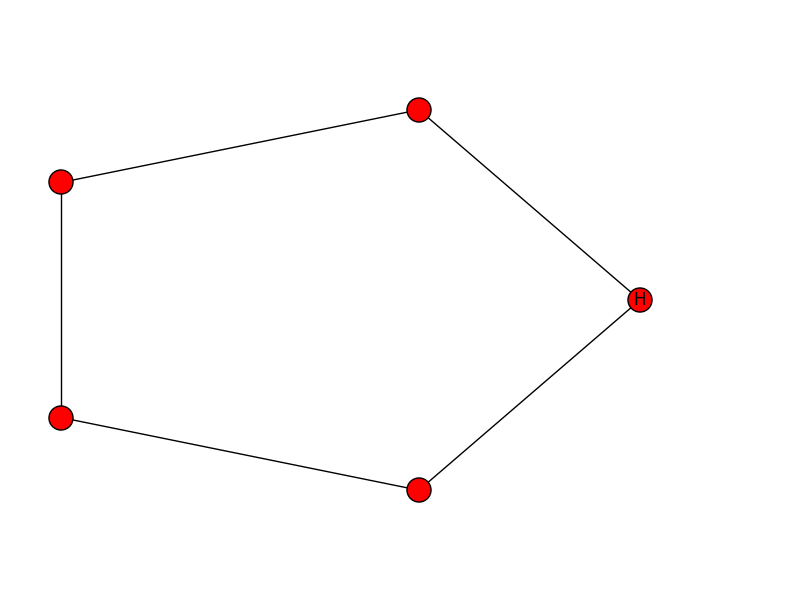
\includegraphics[width=0.8\linewidth]{pics/graph.png}
\caption{Network topology used in the experiments.}
\label{fig1}
\end{figure}


%definition of each variable
%phi -> defined as eq \labe{opinion_sat} and $\phi_i(0) = 0.5$.
%alpha, beta = 0.1
%satisfaction index = 0.5


\subsection{Experiment 1 - Different Allocation Policies}


The first experiment consist of iterating over the four allocation policies (average fair, head first, random order and ration) and compute the evolution of the perceptions ($\Phi(t)$).

Figure \ref{Exp1_half} show the metrics obtained when each turn there are resources available to half of the total demand. Figure \ref{Exp1_single} simulates a more extreme case, where there is resource available only to one of the agents demand, at each turn.


% \begin{figure}
%     \centering
%     \subfloat{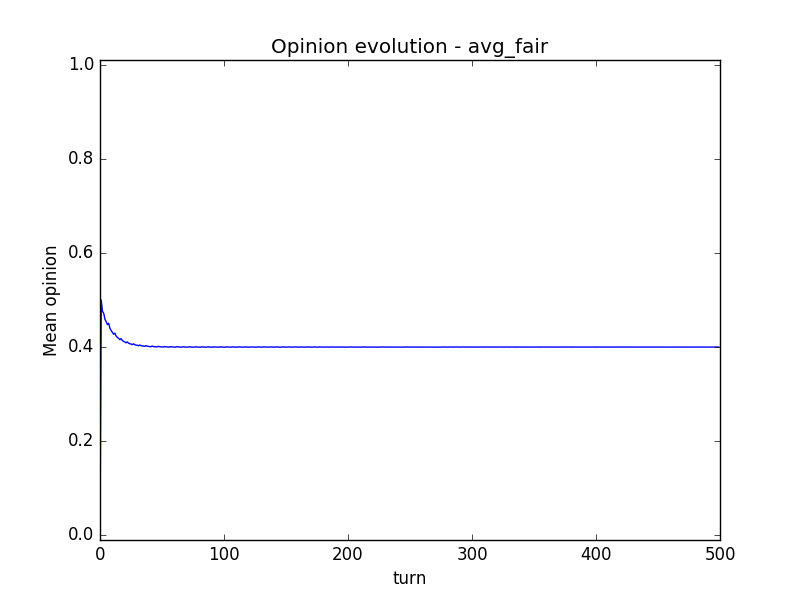
\includegraphics[width=0.8\linewidth]{pics/avg_fair0_5.png}}
%     \\
%     \subfloat{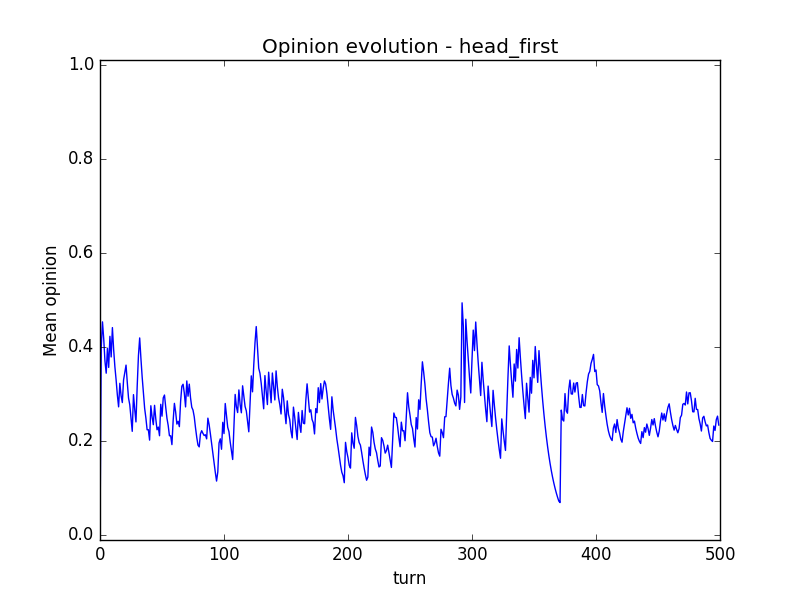
\includegraphics[width=0.8\linewidth]{pics/head_first0_5.png}}
%     \\
%     \subfloat{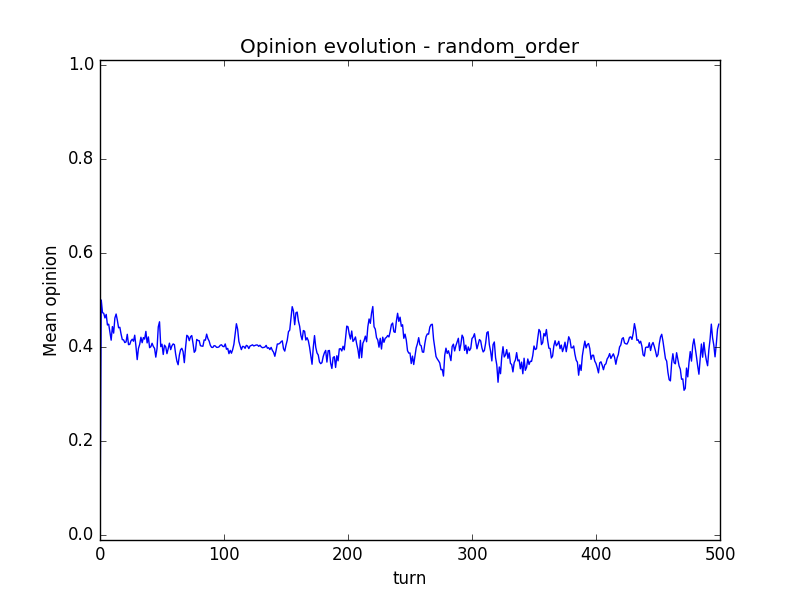
\includegraphics[width=0.8\linewidth]{pics/random_order0_5.png}}
%     \\
%     \subfloat{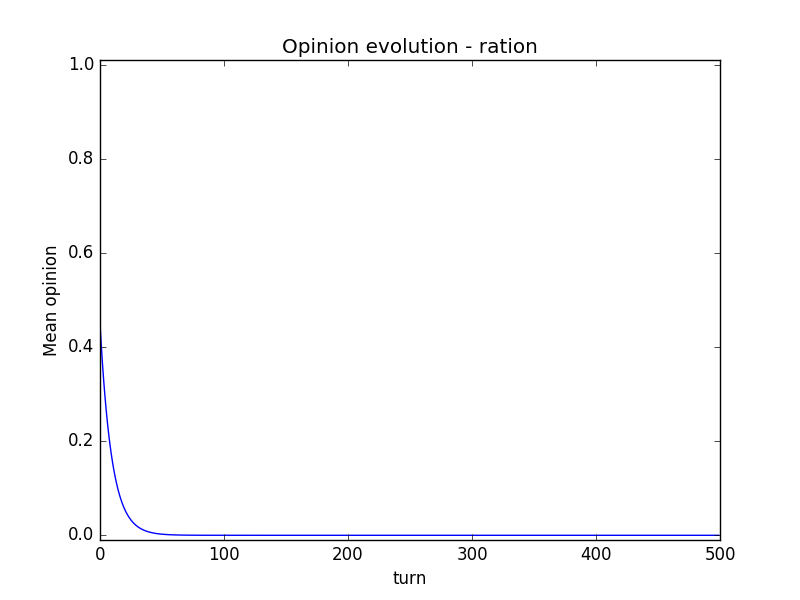
\includegraphics[width=0.8\linewidth]{pics/ration0_5.png}}
%     \caption{Mean opinion for different allocation policies, over time, in an environment with resources enough to half of the agents.}
%     \label{Exp1_half}
% \end{figure}



% \begin{figure}
%     \centering
%     \subfloat{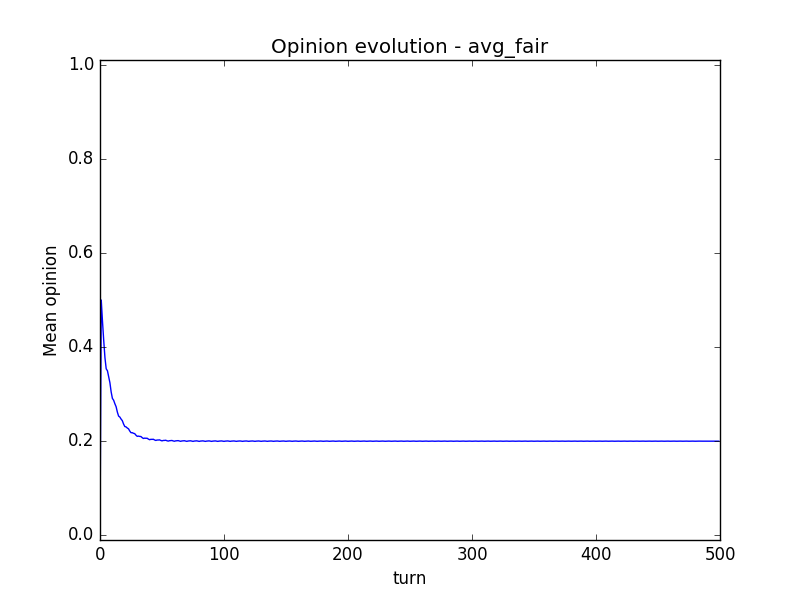
\includegraphics[width=0.8\linewidth]{pics/avg_fair1.png}}
%     \\
%     \subfloat{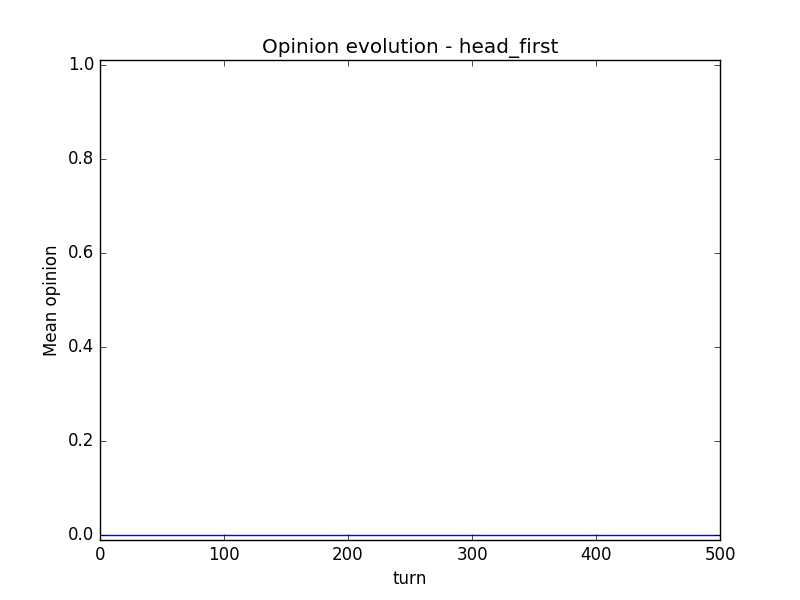
\includegraphics[width=0.8\linewidth]{pics/head_first1.png}}
%     \\
%     \subfloat{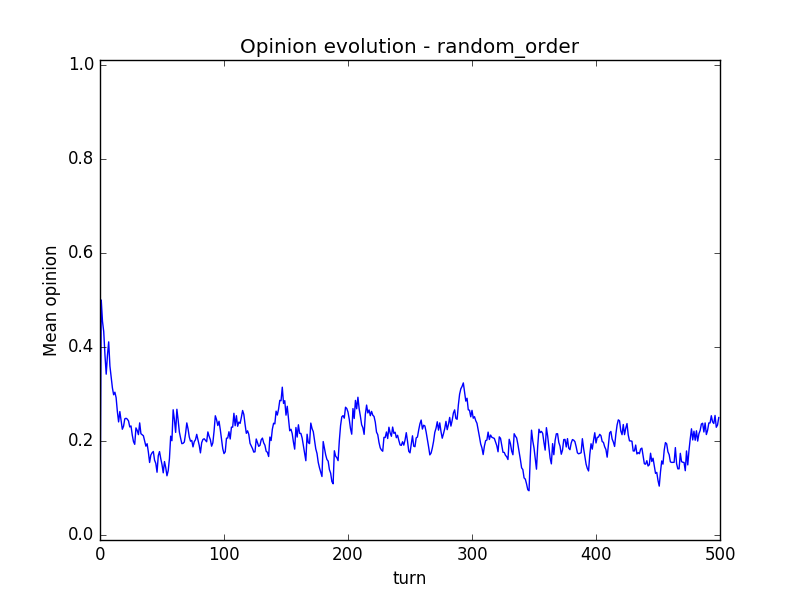
\includegraphics[width=0.8\linewidth]{pics/random_order1.png}}
%     \\
%     \subfloat{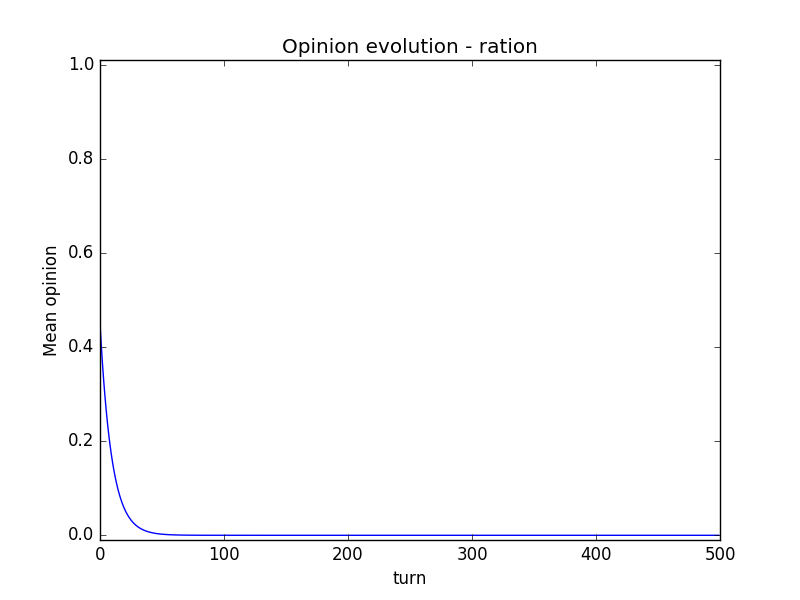
\includegraphics[width=0.8\linewidth]{pics/ration1.png}}
%     \caption{Mean opinion for different allocation policies, over time, in an environment with resources enough to just one agent.}
%     \label{Exp1_single}
% \end{figure}


Figure \ref{Exp1_individual} presents the progression of individuals progressions, with and without effect of social influence. Note that, when there is social influence, in case of unfairness (as is the case), even satisfied agents stop trusting themselves, resulting in general low satisfaction.

% \begin{figure}
%     \centering
%     \subfloat{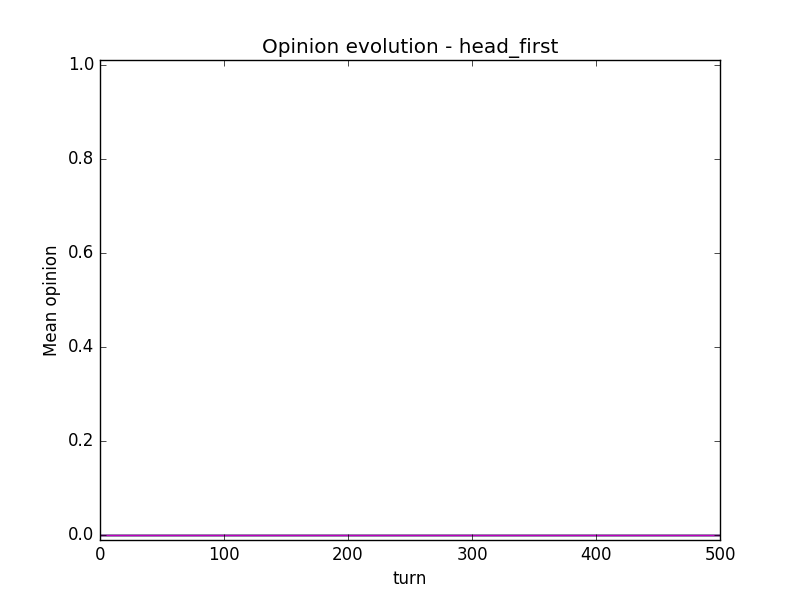
\includegraphics[width=0.8\linewidth]{pics/head_firstmultiple_satisfactions.png}}
%     \\
%     \subfloat{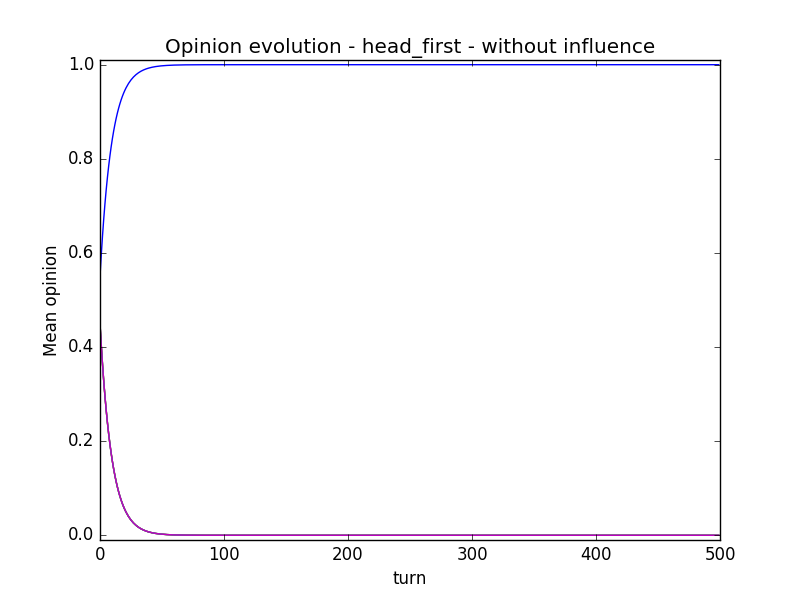
\includegraphics[width=0.8\linewidth]{pics/head_firstoriginal_opinions.png}}
%     \caption{Opinions of every member of the network over time, with and without influence.}
%     \label{Exp1_individual}
% \end{figure}


\subsection{Experiment 2 - Misbehaviour}

In this stage, we simulate a scenario where, despite the presence of a fair allocation (average fair), a single agent always give a negative feedback.

Figure \ref{Exp2_individual} show the evolution of individual opinions, in a scenario without influence propagation. Interestingly, when there is propagation of opinions, the cheating opinion is suppressed, dominating only the coherent opinions, as shown in Figures \ref{Exp2_individual_influence} and \ref{Exp2_average}.

% \begin{figure}
%     \centering
%     \subfloat[Individual opinions, without influence.]{%
%         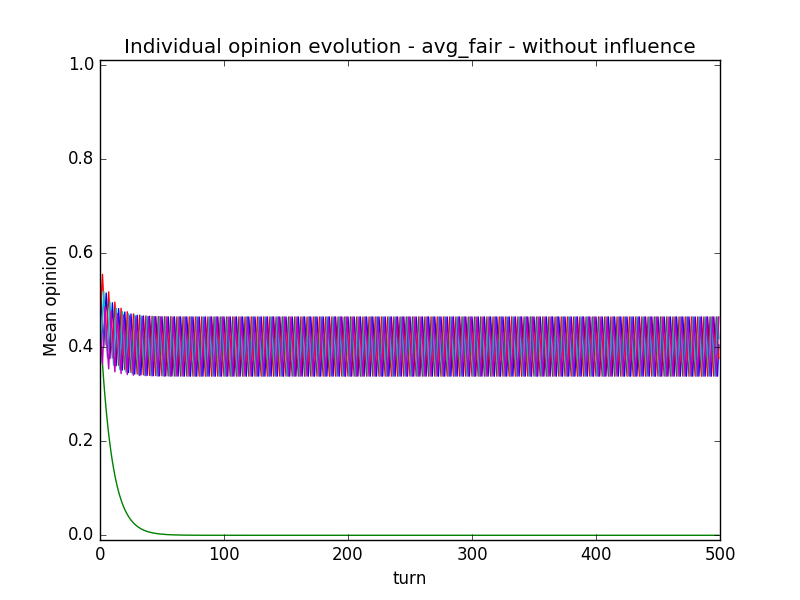
\includegraphics[width=0.8\linewidth]{pics/avg_fair_original_cheat.png}%
%         \label{Exp2_individual}}
%     \\
%     \subfloat[Individual opinions, with influence.]{%
%         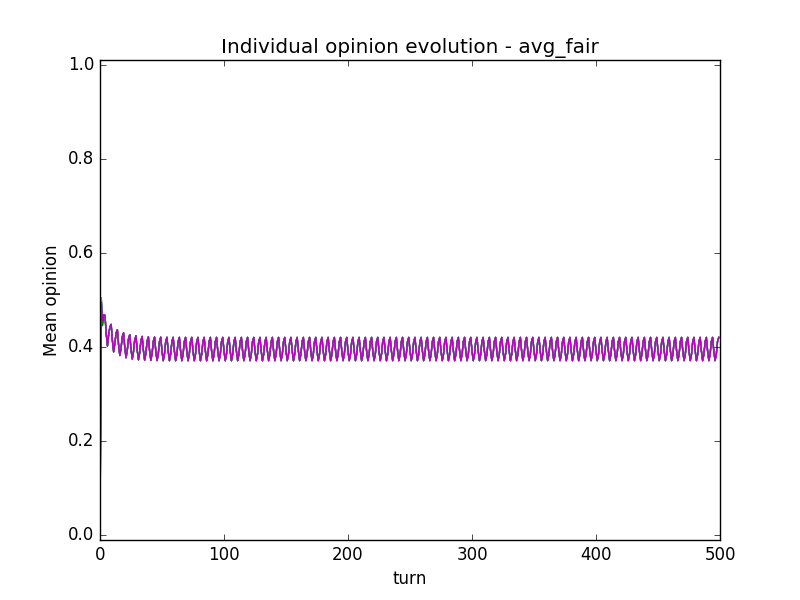
\includegraphics[width=0.8\linewidth]{pics/avg_fair_individual_cheat.png}%
%         \label{Exp2_individual_influence}}
%     \\
%     \subfloat[Mean opinions.]{%
%         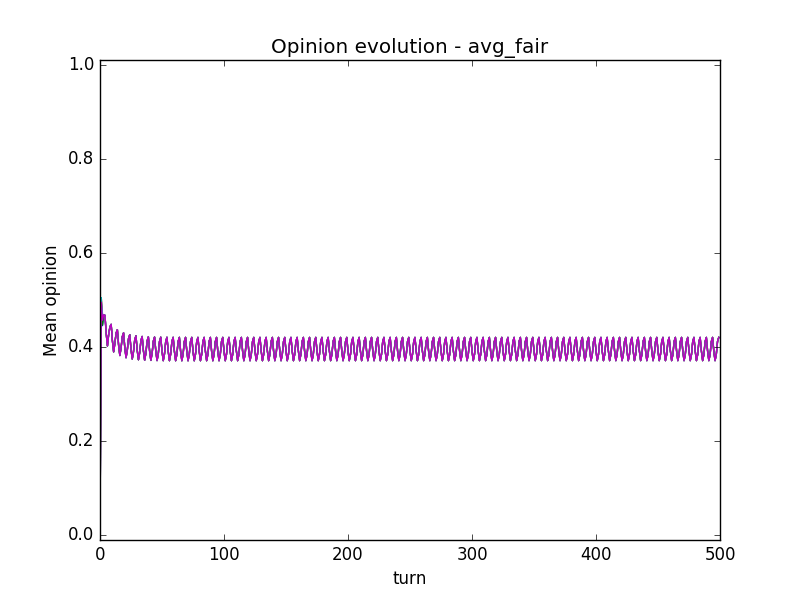
\includegraphics[width=0.8\linewidth]{pics/avg_fair_cheat.png}%
%         \label{Exp2_average}}
%     \caption{Simulations with the presence of a cheating agent, that is always unsatisfied with the allocation, no matter how fair it is.}
%     \label{Exp2}
% \end{figure}


% \subsection{Experiment 3 - Self-Organisation}

% Another experiment is proposed, in order to verify the outcome of a resource allocation, that takes into consideration the direct opinion of the agents and its reputation. 


% Given an agent opinions $\phi_i$ and its \emph{reputation} $\bar{T_i}$, defined as $\bar{T_i} = \frac{1}{n} \sum_{j=1}^{n} T_{ji}$, it is possible to define an \emph{need index} $\eta_i$ defined as:
% $$\eta_i = (1 - \phi_i) \cdot \bar{T_i}$$.

% We then sort all agents by decreasing need index and use this order to allocate resources.

% Figure \ref{Exp3} show that the allocation works properly, when all agents are truthful, generating a fair and sustainable allocation. Figure \ref{Exp3a} shows how, in such regime, the individual opinions remain in a constant and uniform value with small oscillations, revealing the general perception of fairness in the environment. Figure \ref{Exp3b} confirms this, by showing that every individual receives the same amount of resources over time.

% Figure \ref{Exp3Cheat}, however, shows the distribution in a scenario where one agent is cheating, as in the previous experiment. Interestingly, the network is able to detect the individual cheating and, by decreasing its reputation prevent it from receiving any resources. 

% Figure \ref{Exp3Cheata} depicts the cheating behaviour, where Agent 0 (the cheater) has a negative opinion ($\phi_0 = 0$) throughout the whole experiment, independently of the allocation. Figure \ref{Exp3Cheatb} demonstrate the network answer to this behaviour: although initially Agent 0 might receive some resources given its dissatisfaction, after less than 100 turns, its reputation is so low that he stop receiving any resources until the end of the simulation's execution.

% To validate this behaviour in bigger networks, the same tests were performed in a network with 100 agents. Without cheating agents, the scheme was able to produce a fair and sustainable allocation, similar to the one presented in Figure \ref{Exp3}. Also, the presence of cheating agents could be detected and opposed as in the smaller case.

% In order to test the network's ability of detecting cheating agents, a experiment was proposed where the number of cheaters in the network is gradually increased, reaching 50\% of the total number of agents. Figure \ref{Exp3100-2prog} present the results for various numbers of cheating agents.

% It is interesting to notice that until 10 cheaters, the network is able to identify and punish (by starvation) all the cheating agents. When this number is increased to 20 or higher, some cheating agents are successfully identified and punished, but others are not detected and take advantage of more resources than average.

% The reason for this behaviour can be that, when in an environment with abundance of cheaters, compliant agents lose their sense of fairness and can not detect clearly the cheating behaviour and decrease its trust on them. Also, if cheating agents are connected, they will identify with each other and generate trust, mutually increasing their reputations.

% One measure able to oppose this behaviour is to increase agents connections. When an agent have more connections, their notion of the environment can be improved, as there is more information available. 

% This test was performed, by increasing the number of connections of each individual from 2 to 10. Figure \ref{Exp3100-2prog} present the results obtained. As it can be seen, a network where users are more conected is able to identify a bigger number of cheating individuals (up to 30\%, in the results presented). 


%TODO: fazer tabela comparando numero de conexoes e 



% \begin{figure}
%     \centering
%     \subfloat[Individual opinions, without influence.]{%
%         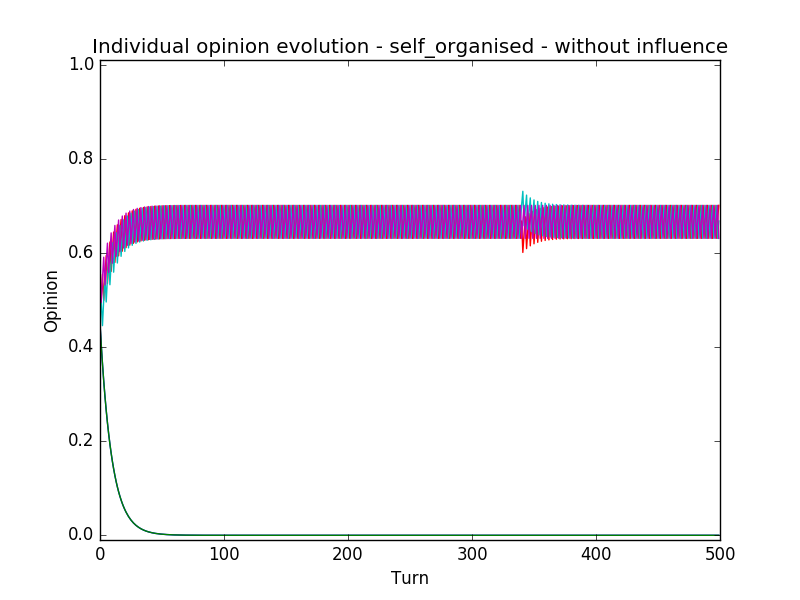
\includegraphics[width=1.0\linewidth]{pics/self_organised_original_cheat.png}%
%         \label{Exp3c_individual}}
%     \\
%     \subfloat[Individual opinions, with influence.]{%
%         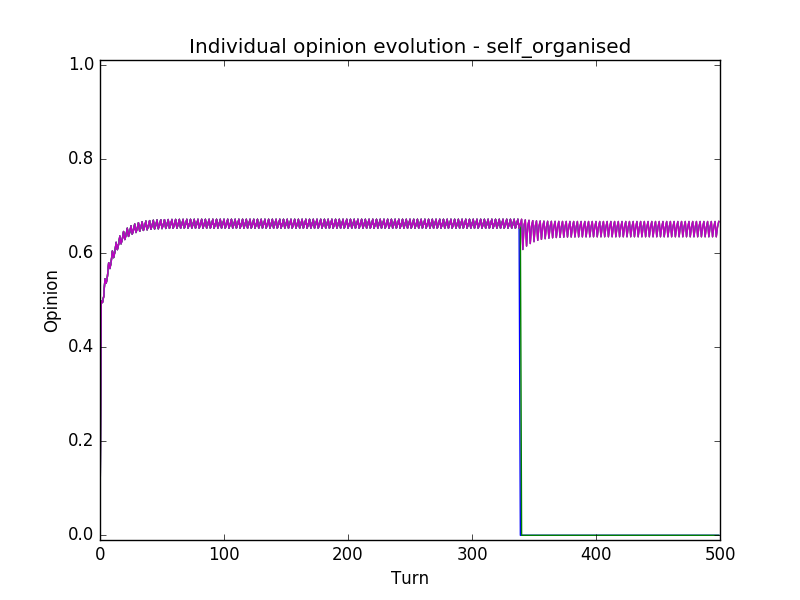
\includegraphics[width=\linewidth]{pics/self_organised_individual_cheat.png}%
%         \label{Exp3c_individual_influence}}
%     \\
%     \subfloat[Mean opinions.]{%
%         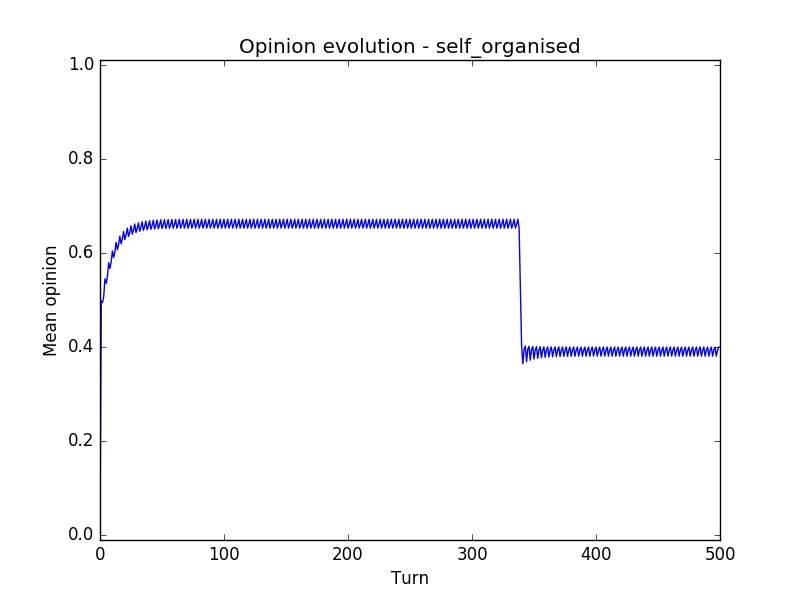
\includegraphics[width=\linewidth]{pics/self_organised_cheat.png}%
%         \label{Exp3c_average}}
%     \caption{Simulations with allocation using need index $\eta_i$, with one agent always complaining regardless the allocation (cheating).}
%     \label{Exp3Cheat}
% \end{figure}

%\subsection{Experiment 4 - Topology} %?

\section{Conclusion}

In this work, a practical method of evaluation of an allocation fairness was developed, using subjective assessments and information diffusion and influence methods.

The solution obtained seems promising, as it allows:

\begin{itemize}
    \item Decentralised and independent computation of an allocation fairness;
    \item Rapid reaction in case of unfairness -- even when there is initial divergence of opinions;
    \item Identification and exclusion of faulty behaviour (cheating);
    \item Perspective of self-organising policies for resource allocation.
\end{itemize}



%TODO: 
%comparacao trusts
%experimentos
%graficos alternativos
%ver questao de atualizar a impressão



% An example of a floating figure using the graphicx package.
% Note that \label must occur AFTER (or within) \caption.
% For figures, \caption should occur after the \includegraphics.
% Note that IEEEtran v1.7 and later has special internal code that
% is designed to preserve the operation of \label within \caption
% even when the captionsoff option is in effect. However, because
% of issues like this, it may be the safest practice to put all your
% \label just after \caption rather than within \caption{}.
%
% Reminder: the "draftcls" or "draftclsnofoot", not "draft", class
% option should be used if it is desired that the figures are to be
% displayed while in draft mode.
%
%\begin{figure}[!t]
%\centering
%\includegraphics[width=2.5in]{myfigure}
% where an .eps filename suffix will be assumed under latex, 
% and a .pdf suffix will be assumed for pdflatex; or what has been declared
% via \DeclareGraphicsExtensions.
%\caption{Simulation results for the network.}
%\label{fig_sim}
%\end{figure}

% Note that the IEEE typically puts floats only at the top, even when this
% results in a large percentage of a column being occupied by floats.


% An example of a double column floating figure using two subfigures.
% (The subfig.sty package must be loaded for this to work.)
% The subfigure \label commands are set within each subfloat command,
% and the \label for the overall figure must come after \caption.
% \hfil is used as a separator to get equal spacing.
% Watch out that the combined width of all the subfigures on a 
% line do not exceed the text width or a line break will occur.
%
%\begin{figure*}[!t]
%\centering
%\subfloat[Case I]{\includegraphics[width=2.5in]{box}%
%\label{fig_first_case}}
%\hfil
%\subfloat[Case II]{\includegraphics[width=2.5in]{box}%
%\label{fig_second_case}}
%\caption{Simulation results for the network.}
%\label{fig_sim}
%\end{figure*}
%
% Note that often IEEE papers with subfigures do not employ subfigure
% captions (using the optional argument to \subfloat[]), but instead will
% reference/describe all of them (a), (b), etc., within the main caption.
% Be aware that for subfig.sty to generate the (a), (b), etc., subfigure
% labels, the optional argument to \subfloat must be present. If a
% subcaption is not desired, just leave its contents blank,
% e.g., \subfloat[].


% An example of a floating table. Note that, for IEEE style tables, the
% \caption command should come BEFORE the table and, given that table
% captions serve much like titles, are usually capitalized except for words
% such as a, an, and, as, at, but, by, for, in, nor, of, on, or, the, to
% and up, which are usually not capitalized unless they are the first or
% last word of the caption. Table text will default to \footnotesize as
% the IEEE normally uses this smaller font for tables.
% The \label must come after \caption as always.
%
%\begin{table}[!t]
%% increase table row spacing, adjust to taste
%\renewcommand{\arraystretch}{1.3}
% if using array.sty, it might be a good idea to tweak the value of
% \extrarowheight as needed to properly center the text within the cells
%\caption{An Example of a Table}
%\label{table_example}
%\centering
%% Some packages, such as MDW tools, offer better commands for making tables
%% than the plain LaTeX2e tabular which is used here.
%\begin{tabular}{|c||c|}
%\hline
%One & Two\\
%\hline
%Three & Four\\
%\hline
%\end{tabular}
%\end{table}


% Note that the IEEE does not put floats in the very first column
% - or typically anywhere on the first page for that matter. Also,
% in-text middle ("here") positioning is typically not used, but it
% is allowed and encouraged for Computer Society conferences (but
% not Computer Society journals). Most IEEE journals/conferences use
% top floats exclusively. 
% Note that, LaTeX2e, unlike IEEE journals/conferences, places
% footnotes above bottom floats. This can be corrected via the
% \fnbelowfloat command of the stfloats package.



% use section* for acknowledgment
\ifCLASSOPTIONcompsoc
  % The Computer Society usually uses the plural form
  \section*{Acknowledgments}
\else
  % regular IEEE prefers the singular form
  \section*{Acknowledgment}
\fi

This work is partially supported by the National Council for Scientific and Technological Development (CNPq), Brazil.


% if have a single appendix:
%\appendix[Proof of the Zonklar Equations]
% or
%\appendix  % for no appendix heading
% do not use \section anymore after \appendix, only \section*
% is possibly needed

% use appendices with more than one appendix
% then use \section to start each appendix
% you must declare a \section before using any
% \subsection or using \label (\appendices by itself
% starts a section numbered zero.)
%


% trigger a \newpage just before the given reference
% number - used to balance the columns on the last page
% adjust value as needed - may need to be readjusted if
% the document is modified later
%\IEEEtriggeratref{8}
% The "triggered" command can be changed if desired:
%\IEEEtriggercmd{\enlargethispage{-5in}}

% references section

% can use a bibliography generated by BibTeX as a .bbl file
% BibTeX documentation can be easily obtained at:
% http://mirror.ctan.org/biblio/bibtex/contrib/doc/
% The IEEEtran BibTeX style support page is at:
% http://www.michaelshell.org/tex/ieeetran/bibtex/
%\bibliographystyle{IEEEtran}
% argument is your BibTeX string definitions and bibliography database(s)
%\bibliography{IEEEabrv,../bib/paper}
%
% <OR> manually copy in the resultant .bbl file
% set second argument of \begin to the number of references
% (used to reserve space for the reference number labels box)
% \begin{thebibliography}{1}

% \bibitem{IEEEhowto:kopka}
% H.~Kopka and P.~W. Daly, \emph{A Guide to \LaTeX}, 3rd~ed.\hskip 1em plus
%   0.5em minus 0.4em\relax Harlow, England: Addison-Wesley, 1999.

% \end{thebibliography}

\bibliographystyle{plain}
\bibliography{jeremy}


\appendix[Figures]
% \section{Exp 1 images}

\begin{figure}
    \centering
    \subfloat{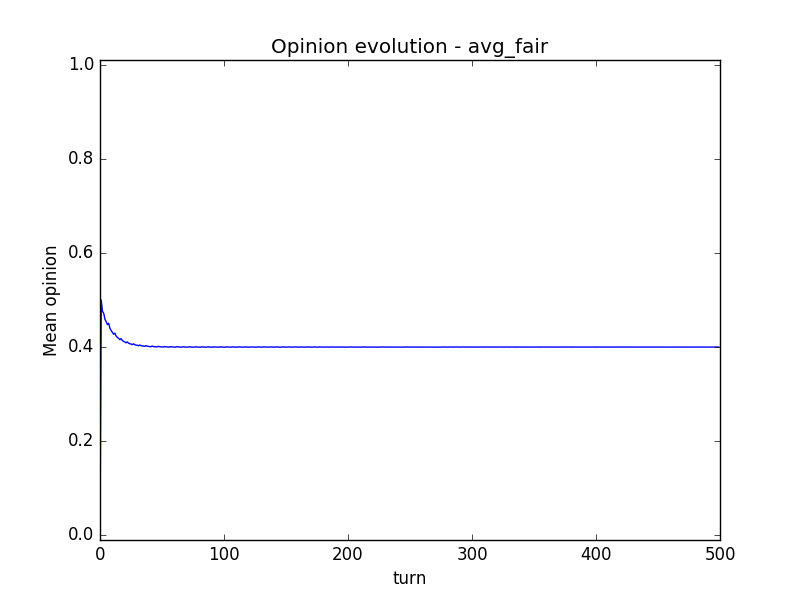
\includegraphics[width=0.8\linewidth]{pics/avg_fair0_5.png}}
    \\
    \subfloat{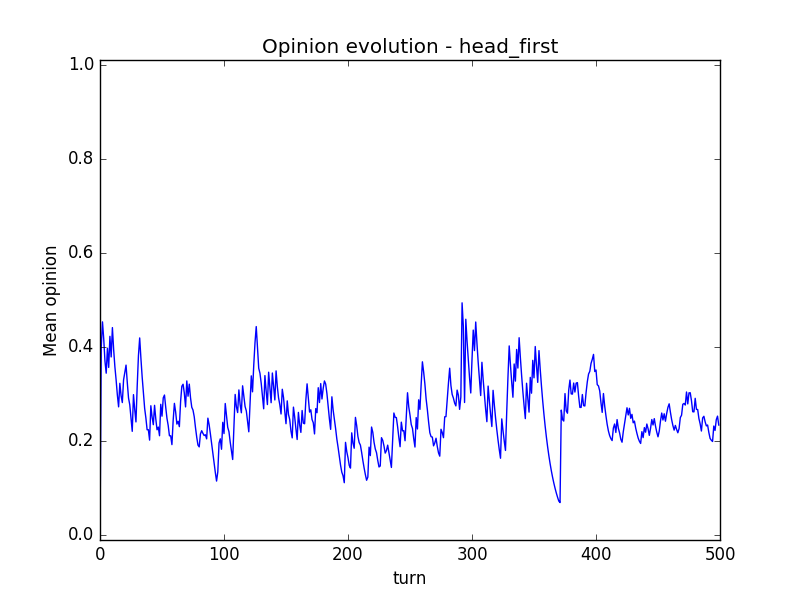
\includegraphics[width=0.8\linewidth]{pics/head_first0_5.png}}
    \\
    \subfloat{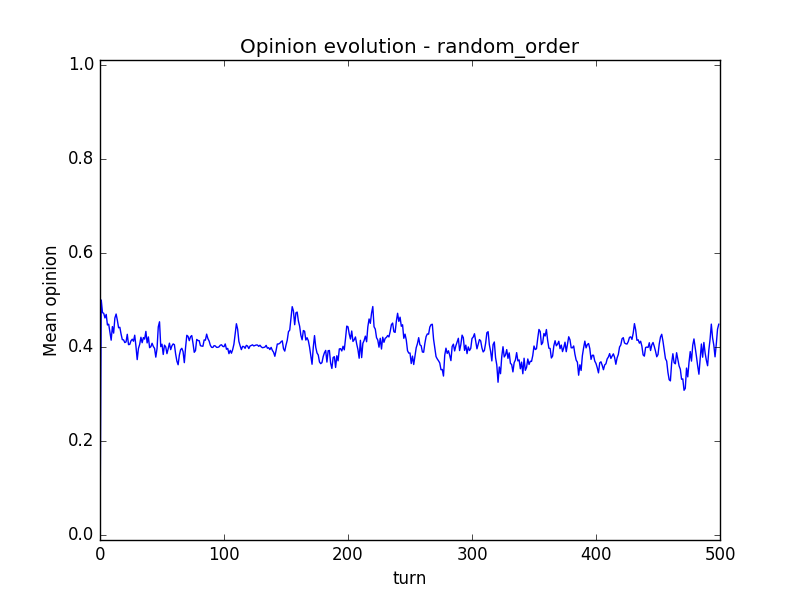
\includegraphics[width=0.8\linewidth]{pics/random_order0_5.png}}
    \\
    \subfloat{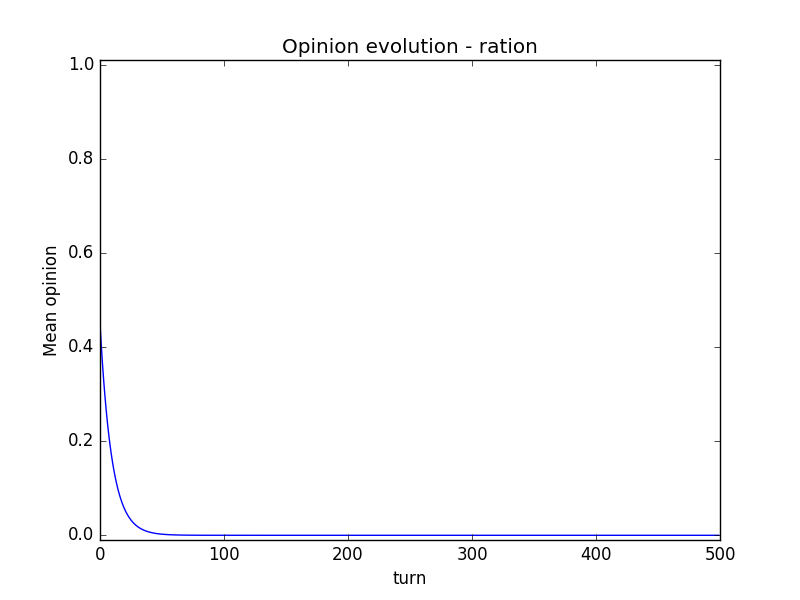
\includegraphics[width=0.8\linewidth]{pics/ration0_5.png}}
    \caption{Mean opinion for different allocation policies, over time, in an environment with resources enough to half of the agents.}
    \label{Exp1_half}
\end{figure}



\begin{figure}
    \centering
    \subfloat{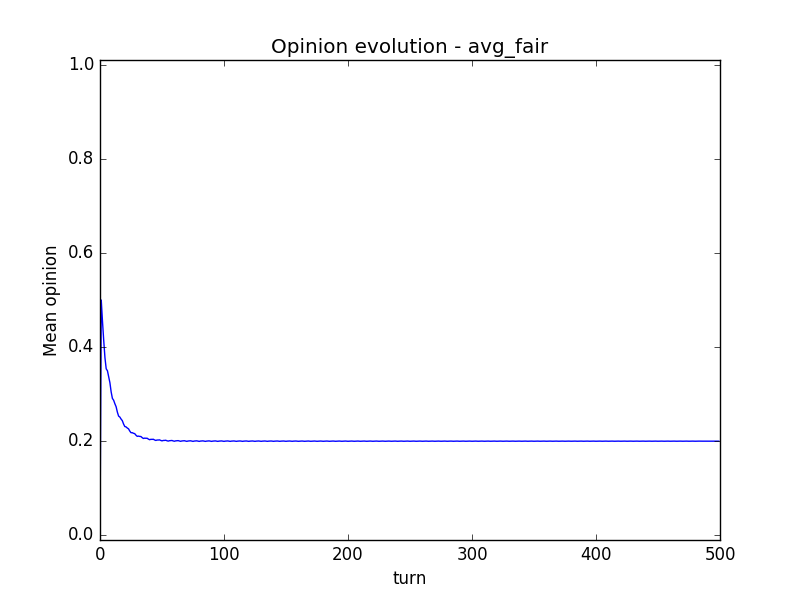
\includegraphics[width=0.8\linewidth]{pics/avg_fair1.png}}
    \\
    \subfloat{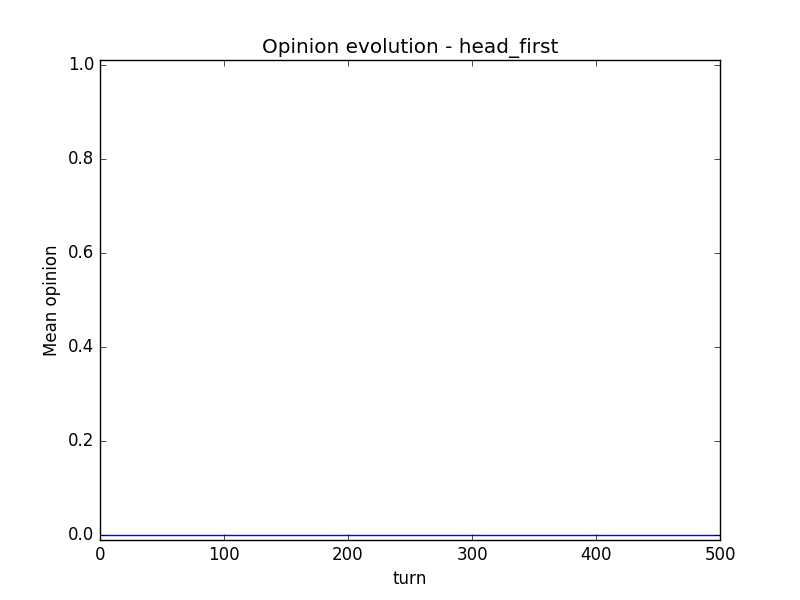
\includegraphics[width=0.8\linewidth]{pics/head_first1.png}}
    \\
    \subfloat{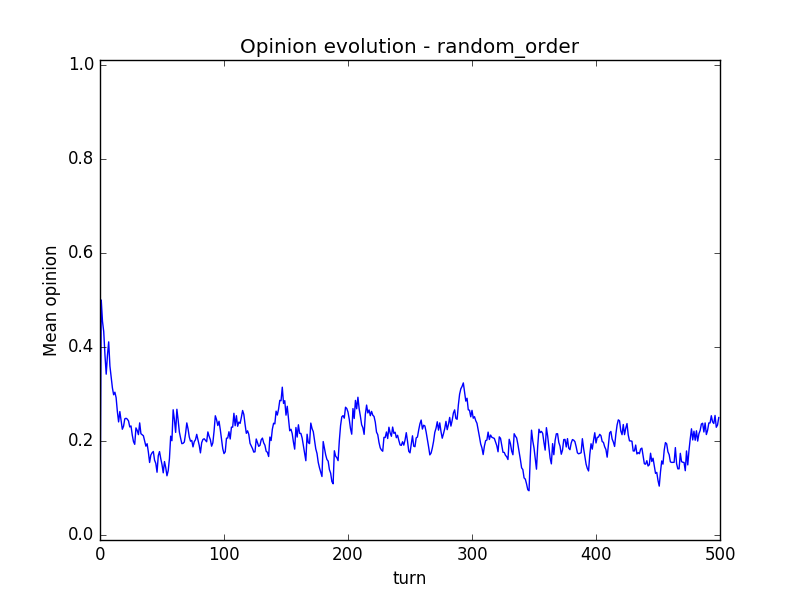
\includegraphics[width=0.8\linewidth]{pics/random_order1.png}}
    \\
    \subfloat{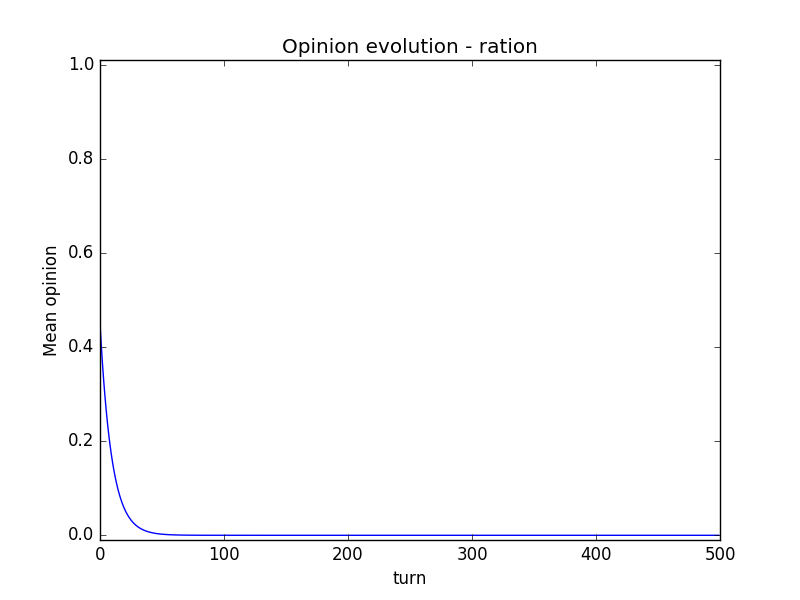
\includegraphics[width=0.8\linewidth]{pics/ration1.png}}
    \caption{Mean opinion for different allocation policies, over time, in an environment with resources enough to just one agent.}
    \label{Exp1_single}
\end{figure}

\begin{figure}
    \centering
    \subfloat{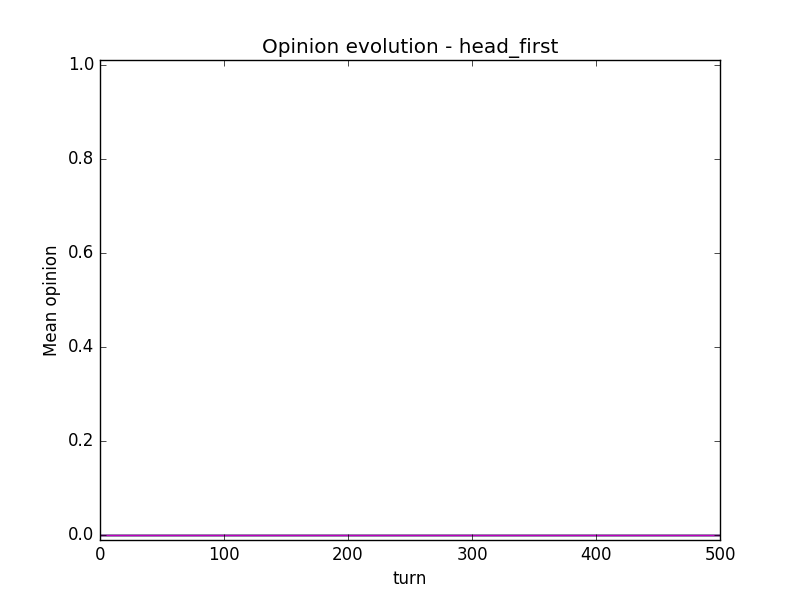
\includegraphics[width=0.8\linewidth]{pics/head_firstmultiple_satisfactions.png}}
    \\
    \subfloat{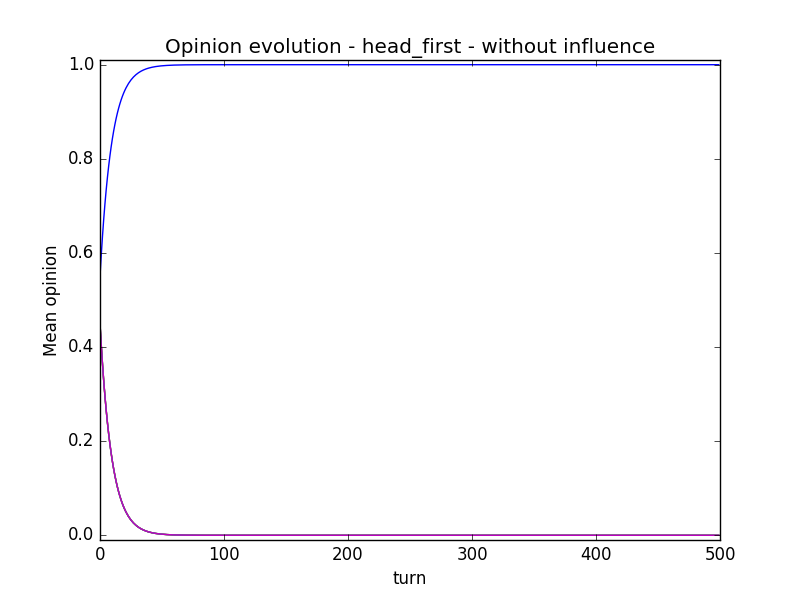
\includegraphics[width=0.8\linewidth]{pics/head_firstoriginal_opinions.png}}
    \caption{Opinions of every member of the network over time, with and without influence.}
    \label{Exp1_individual}
\end{figure}


% \section{Exp 2 Images}

\begin{figure}
    \centering
    \subfloat[Individual opinions, without influence.]{%
        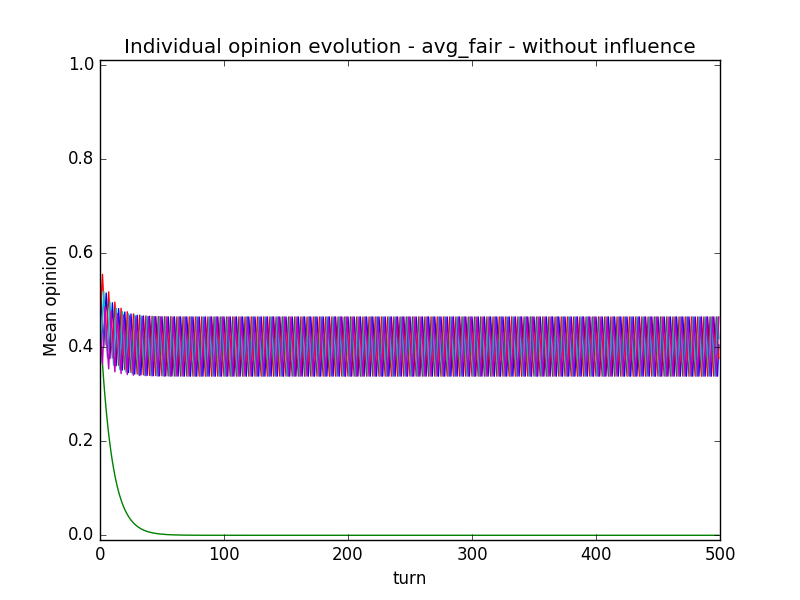
\includegraphics[width=0.8\linewidth]{pics/avg_fair_original_cheat.png}%
        \label{Exp2_individual}}
    \\
    \subfloat[Individual opinions, with influence.]{%
        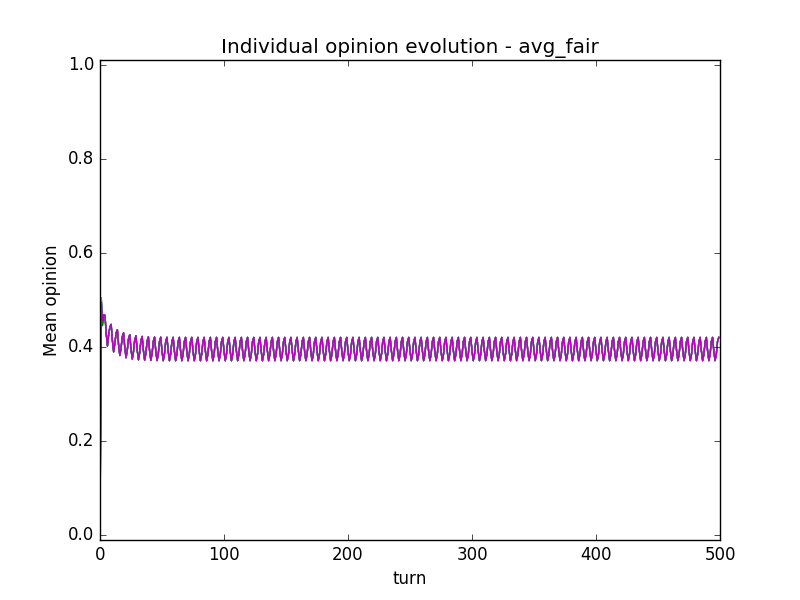
\includegraphics[width=0.8\linewidth]{pics/avg_fair_individual_cheat.png}%
        \label{Exp2_individual_influence}}
    \\
    \subfloat[Mean opinions.]{%
        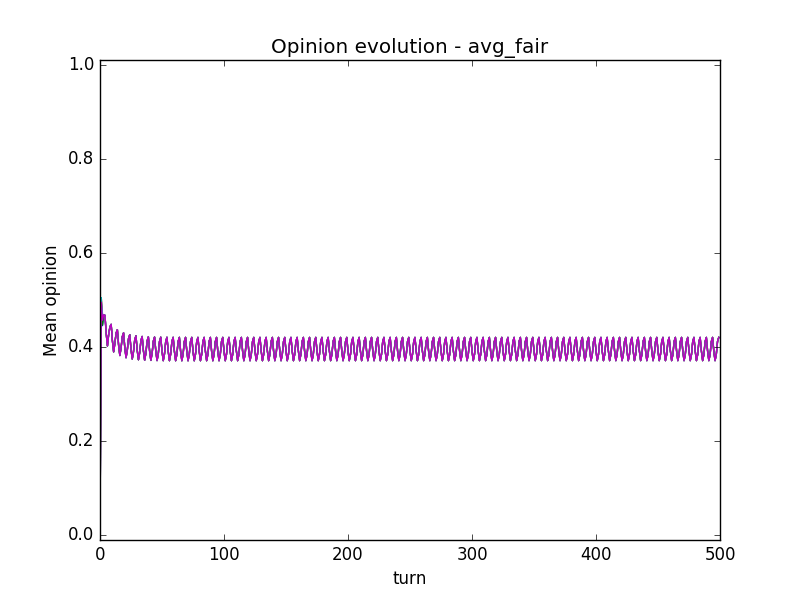
\includegraphics[width=0.8\linewidth]{pics/avg_fair_cheat.png}%
        \label{Exp2_average}}
    \caption{Simulations with the presence of a cheating agent, that is always unsatisfied with the allocation, no matter how fair it is.}
    \label{Exp2}
\end{figure}


% % \section{Exp 3 Images}

% % \begin{figure}
% %     \centering
% %     \subfloat[No cheating, 5 individuals, opinion evolution.]{%
% %         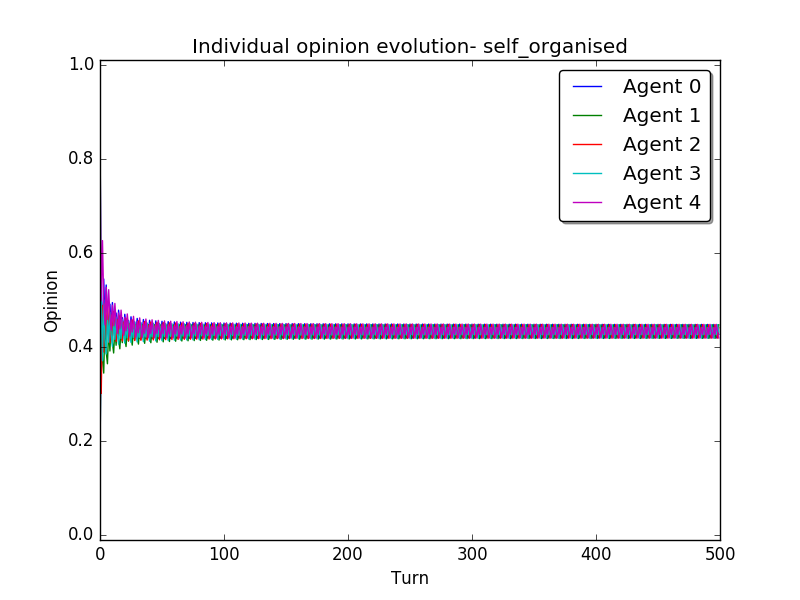
\includegraphics[width=0.8\linewidth]{pics/selforg_0cheaters_2nei_5agents-opinions.png}%
% %         \label{Exp3a}}
% %     \\
% %     \subfloat[No cheating, 5 individuals, allocation evolution.]{%
% %         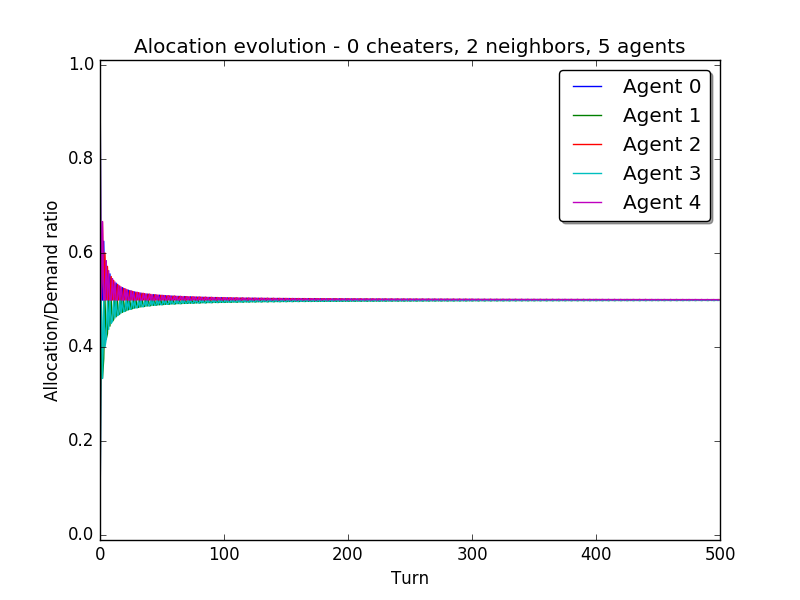
\includegraphics[width=0.8\linewidth]{pics/selforg_0cheaters_2nei_5agents-alloc.png}%
% %         \label{Exp3b}}
% %     \caption{Simulations of self-organising allocation.}
% %     \label{Exp3}
% % \end{figure}    


% \begin{figure}
%     \centering
%     \subfloat{%
%         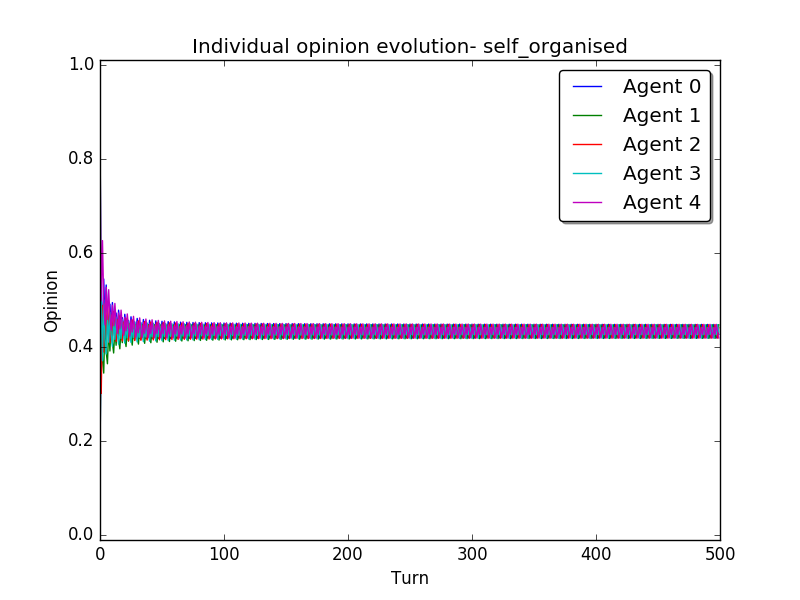
\includegraphics[width=0.7\linewidth]{pics/selforg_0cheaters_2nei_5agents-opinions.png}%
%         \label{Exp3a}}
%     \\
%     \subfloat{%
%         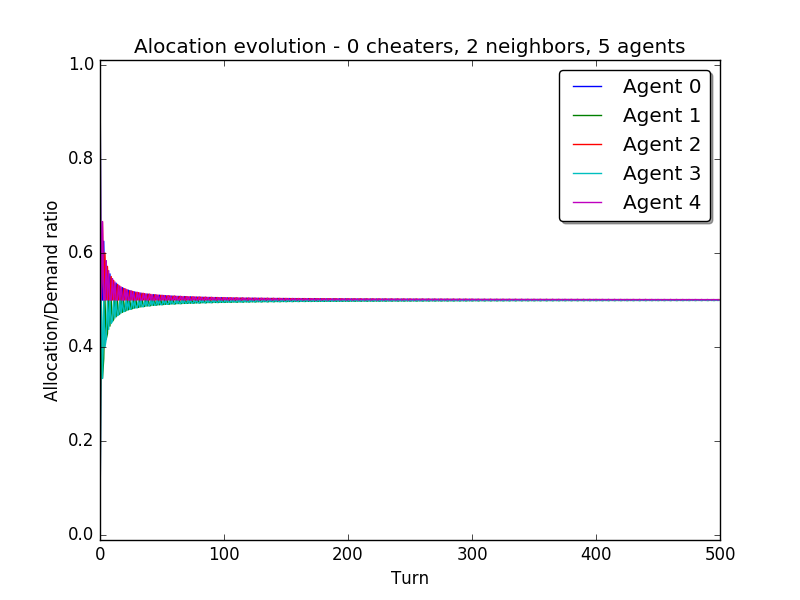
\includegraphics[width=0.7\linewidth]{pics/selforg_0cheaters_2nei_5agents-alloc.png}%
%         \label{Exp3b}}
%     \caption{Simulations of self-organising allocation.}
%     \label{Exp3}
% \end{figure}    

    
% \begin{figure}
%     \centering
%     \subfloat{%
%     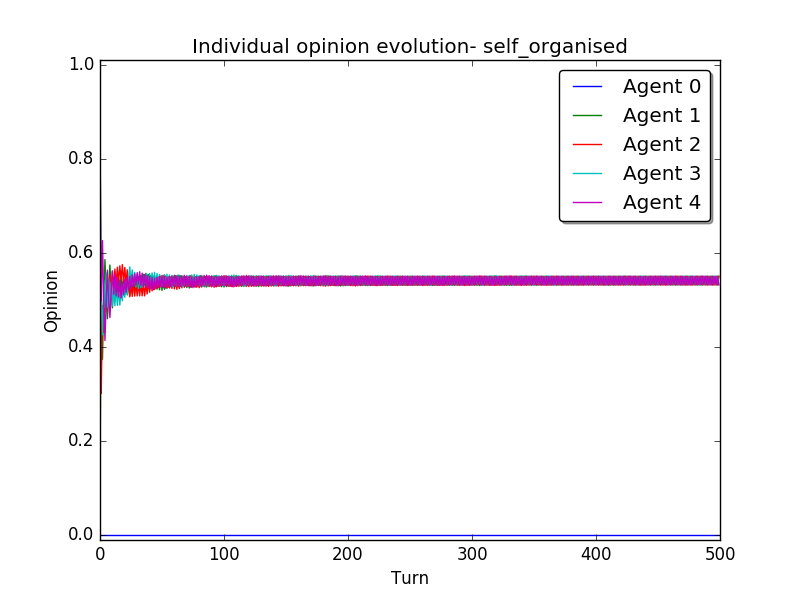
\includegraphics[width=0.7\linewidth]{pics/selforg_1cheaters_2nei_5agents-opinions.png}%
%     \label{Exp3Cheata}}
%     \\
%     \subfloat{%
%         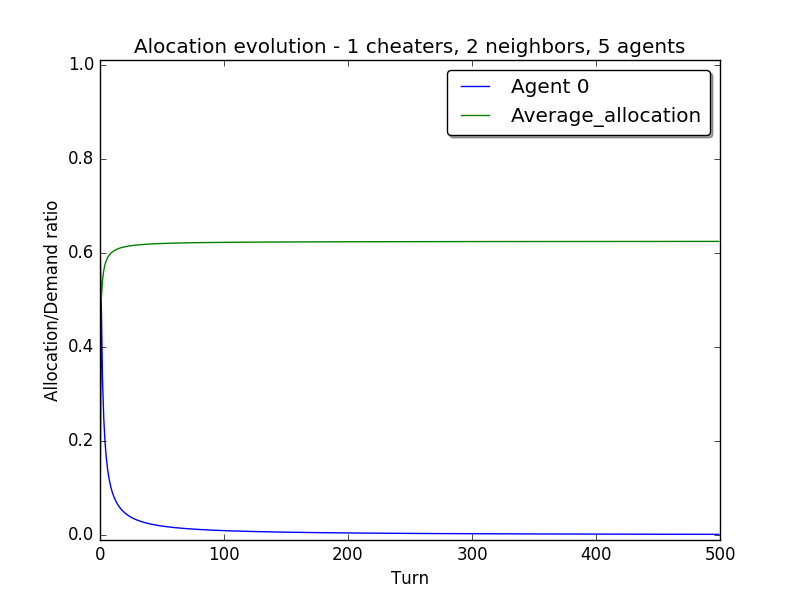
\includegraphics[width=0.7\linewidth]{pics/selforg_1cheaters_2nei_5agents-alloc.png}%
%         \label{Exp3Cheatb}}
%     \caption{Simulations of self-organising allocation, with cheating agent.}
%     \label{Exp3Cheat}
% \end{figure}


% \begin{figure*}
%     \centering
%     \subfloat[1 Cheater]{%
%     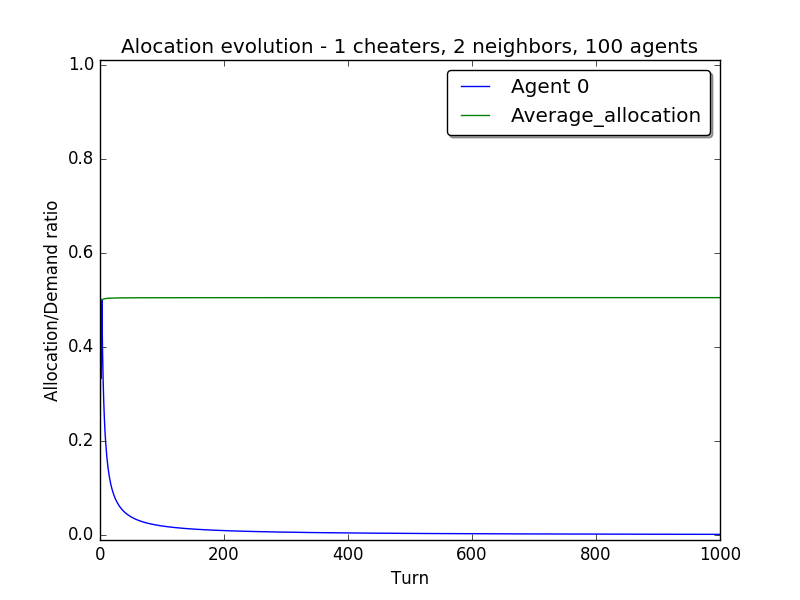
\includegraphics[width=0.4\linewidth]{pics/selforg_1cheaters_2nei_100agents-alloc.png}}
%     ~
%     \subfloat[5 Cheaters]{%
%     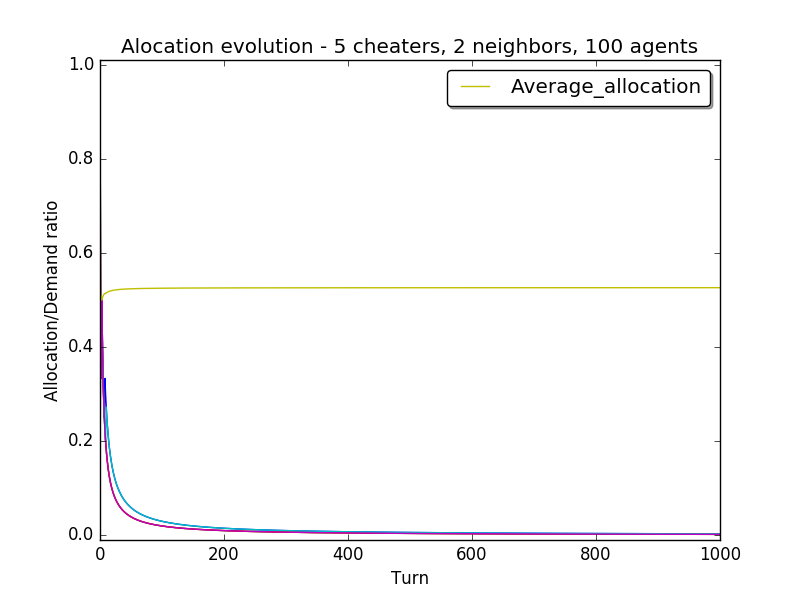
\includegraphics[width=0.4\linewidth]{pics/selforg_5cheaters_2nei_100agents-alloc.png}}
%     \\
%     \subfloat[10 Cheaters]{%
%     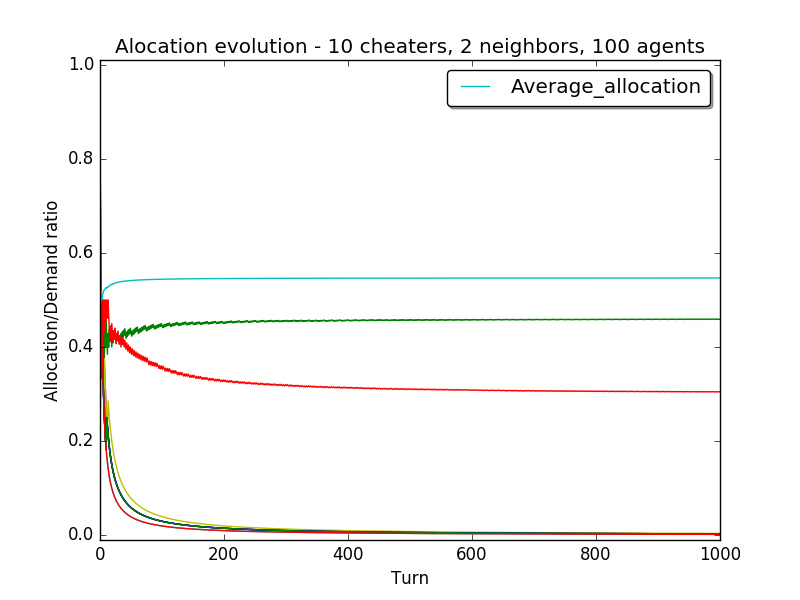
\includegraphics[width=0.4\linewidth]{pics/selforg_10cheaters_2nei_100agents-alloc.png}}
%     ~
%     \subfloat[20 Cheaters]{%
%     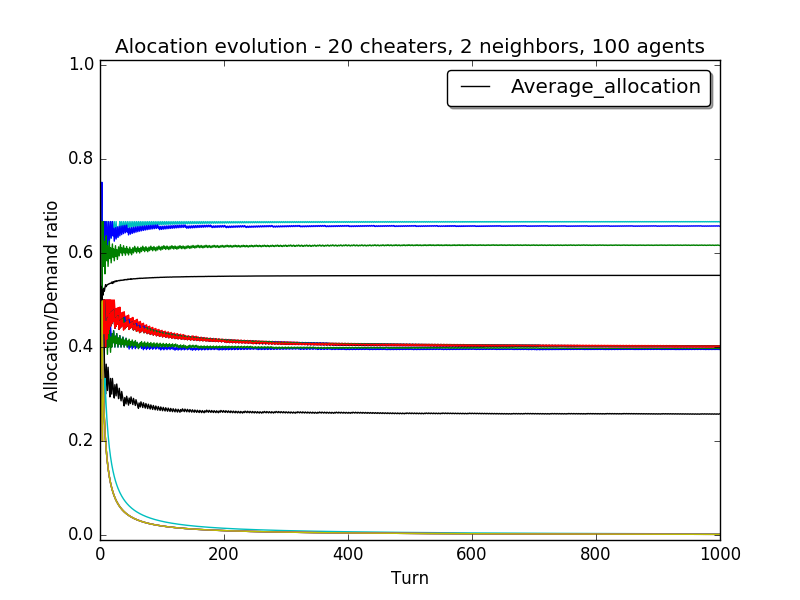
\includegraphics[width=0.4\linewidth]{pics/selforg_20cheaters_2nei_100agents-alloc.png}}
%     \\
%     \subfloat[30 Cheaters]{%
%     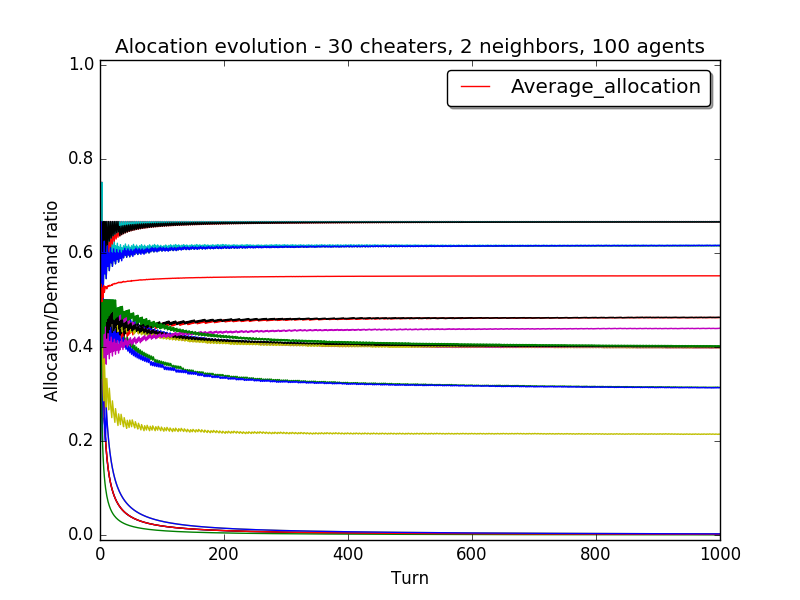
\includegraphics[width=0.4\linewidth]{pics/selforg_30cheaters_2nei_100agents-alloc.png}}
%     ~
%     \subfloat[50 Cheaters]{%
%     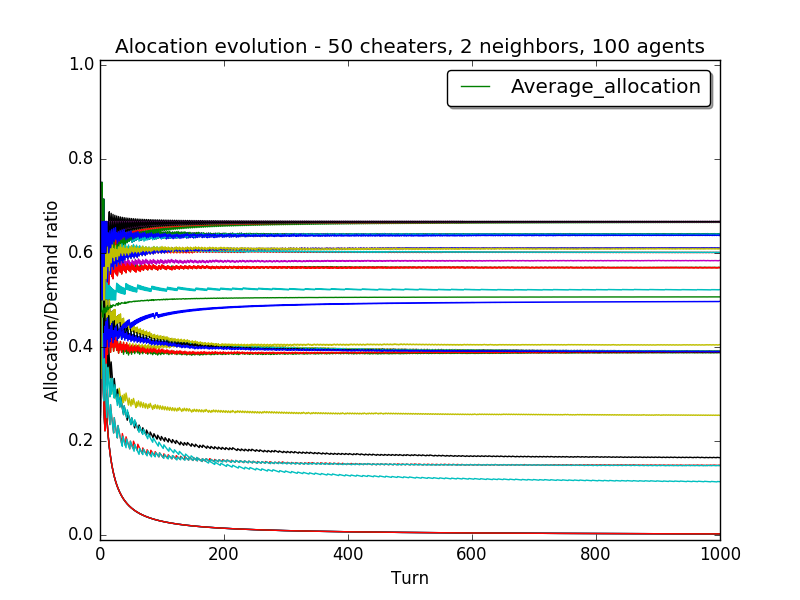
\includegraphics[width=0.4\linewidth]{pics/selforg_50cheaters_2nei_100agents-alloc.png}}
%     \caption{Allocation evolutions for a network with 100 individuals, with 2 connections each (circular ring network). Each image shows a differente number of cheating agents.}
%     \label{Exp3100-2prog}
% \end{figure*}

% \begin{figure*}
%     \centering
%     \subfloat[1 Cheater]{%
%     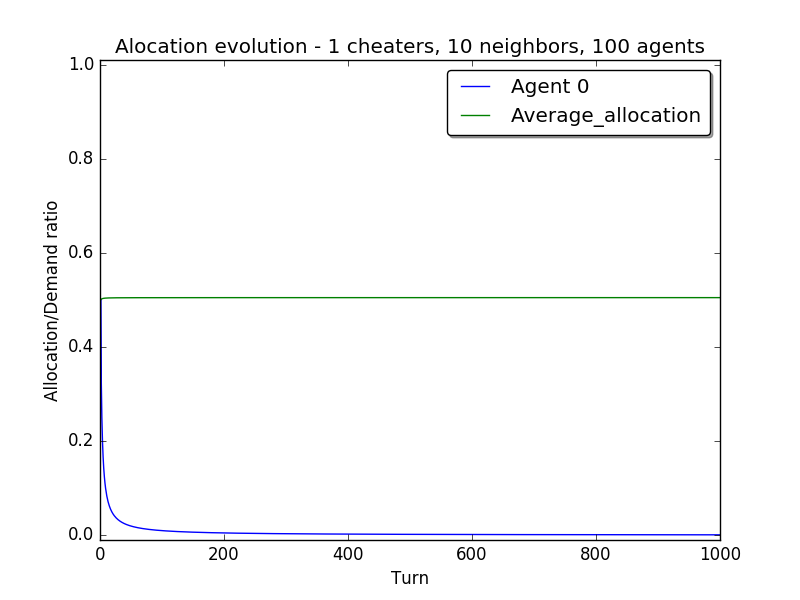
\includegraphics[width=0.4\linewidth]{pics/selforg_1cheaters_10nei_100agents-alloc.png}}
%     ~
%     \subfloat[5 Cheaters]{%
%     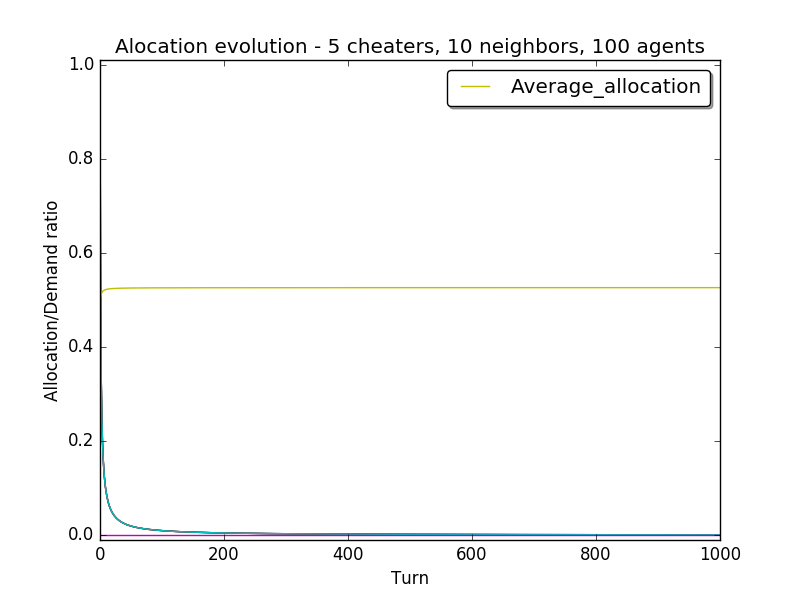
\includegraphics[width=0.4\linewidth]{pics/selforg_5cheaters_10nei_100agents-alloc.png}}
%     \\
%     \subfloat[10 Cheaters]{%
%     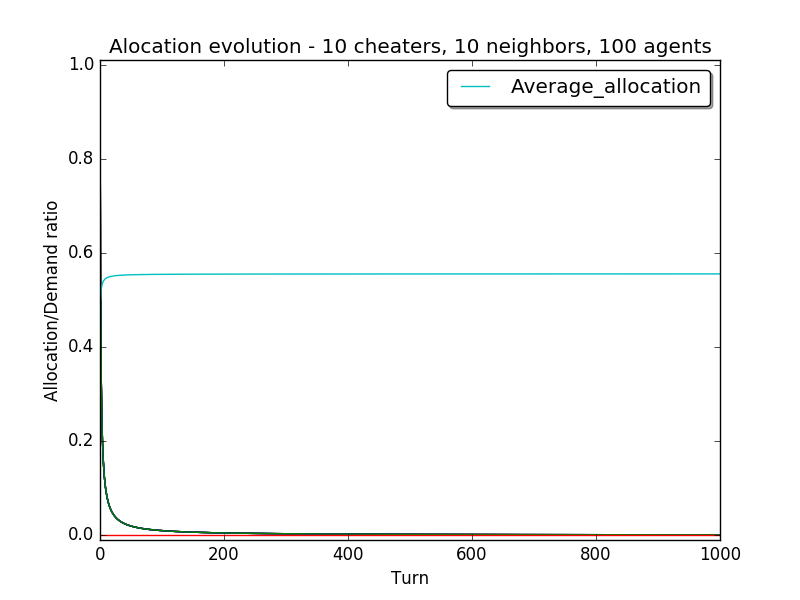
\includegraphics[width=0.4\linewidth]{pics/selforg_10cheaters_10nei_100agents-alloc.png}}
%     ~
%     \subfloat[20 Cheaters]{%
%     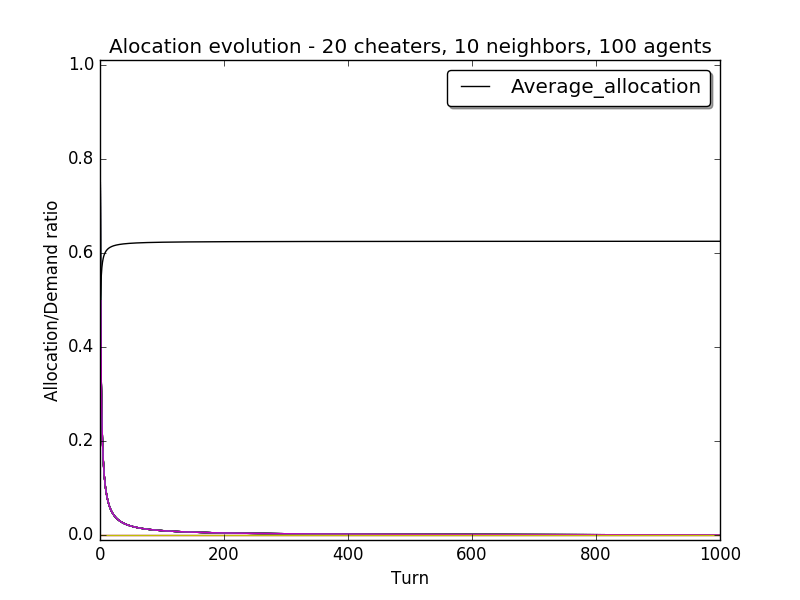
\includegraphics[width=0.4\linewidth]{pics/selforg_20cheaters_10nei_100agents-alloc.png}}
%     \\
%     \subfloat[30 Cheaters]{%
%     \includegraphics[width=0.4\linewidth]{pics/selforg_30cheaters_10nei_100agents-alloc.png}}
%     ~
%     \subfloat[50 Cheaters]{%
%     \includegraphics[width=0.4\linewidth]{pics/selforg_50cheaters_10nei_100agents-alloc.png}}
%     \caption{Same progression as Fig \ref{Exp3100-2prog}, but with each individual having 10 connections in total each.}
%     \label{Exp3100-10prog}
% \end{figure*}


% that's all folks
\end{document}







